% !TeX spellcheck = it_IT
\section{WiFi 802.11}

Lo standard considerato da adesso è 802.11. I requisiti generali sono: 
\begin{itemize}
	\item Throughput maggiore possibile

	\item elevato numero di nodi, gestiti da più celle

	\item connessione verso la dorsale (backbone) cablata

	\item Raggio 100-300m

	\item Utilizzo efficiente (non estremo) della batteria

	\item Più WLAN devono poter coesistere

	\item Operare nelle bande di frequenza unlicensed

	\item Configurazione dinamica (selezione canali, autenticazione)
\end{itemize}

\paragraph{Wireless Fidelity WiFi:} Si ha una rete con \textbf{uno o più Access Point AP}, coordinata da \textbf{Point Coordination Function PCF} (ovvero si ha un solo punto di coordinamento, l'AP). 

Un \textbf{Basic Service Set BSS} identifica la cella o rete WiFi (nome/caratteristiche della rete).
\begin{center}
	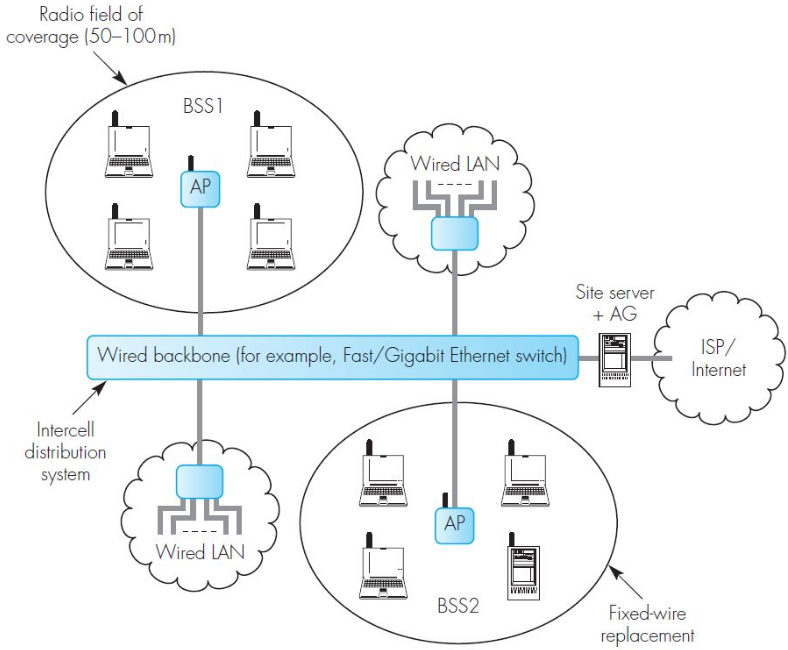
\includegraphics[width=0.7\linewidth]{img/wlan/wifistruct1}
\end{center}

Si può anche avere una \textbf{rete Ad-Hoc}, senza una PCF, ma con una \textbf{Distributed Coordination Function DCF}, con un \textbf{Independent Basic Service Set IBSS}
\begin{center}
	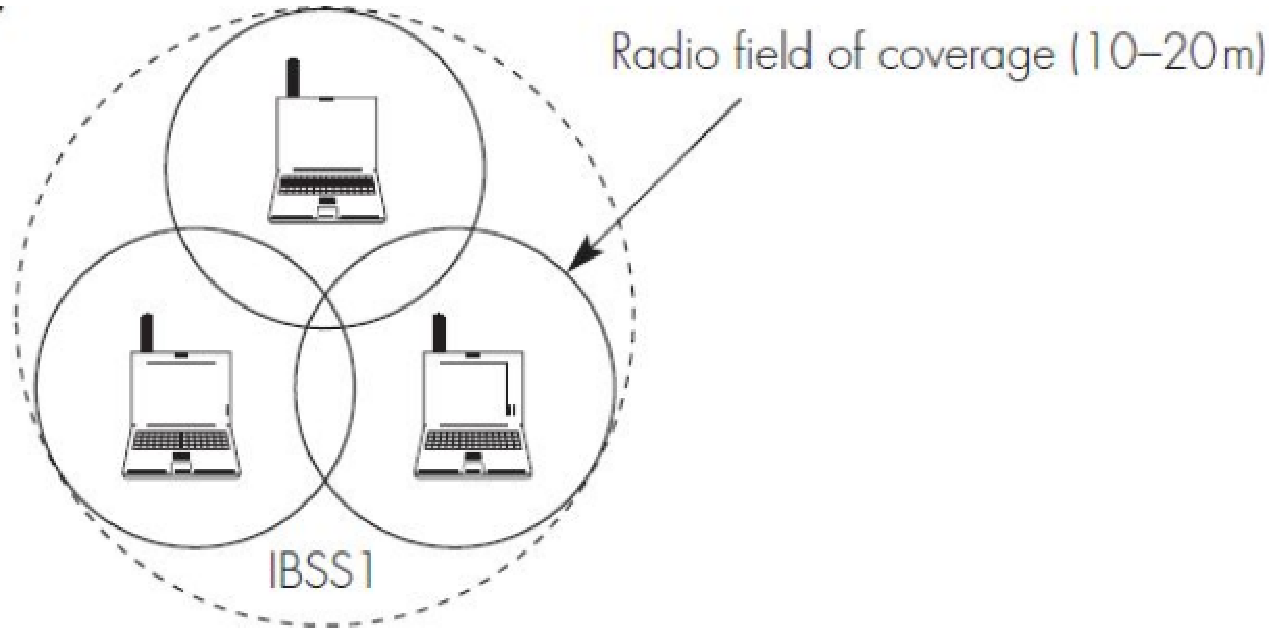
\includegraphics[width=0.45\linewidth]{img/wlan/wifistruct2}
\end{center}

\subsection{Architettura dei protocolli}

\begin{center}
	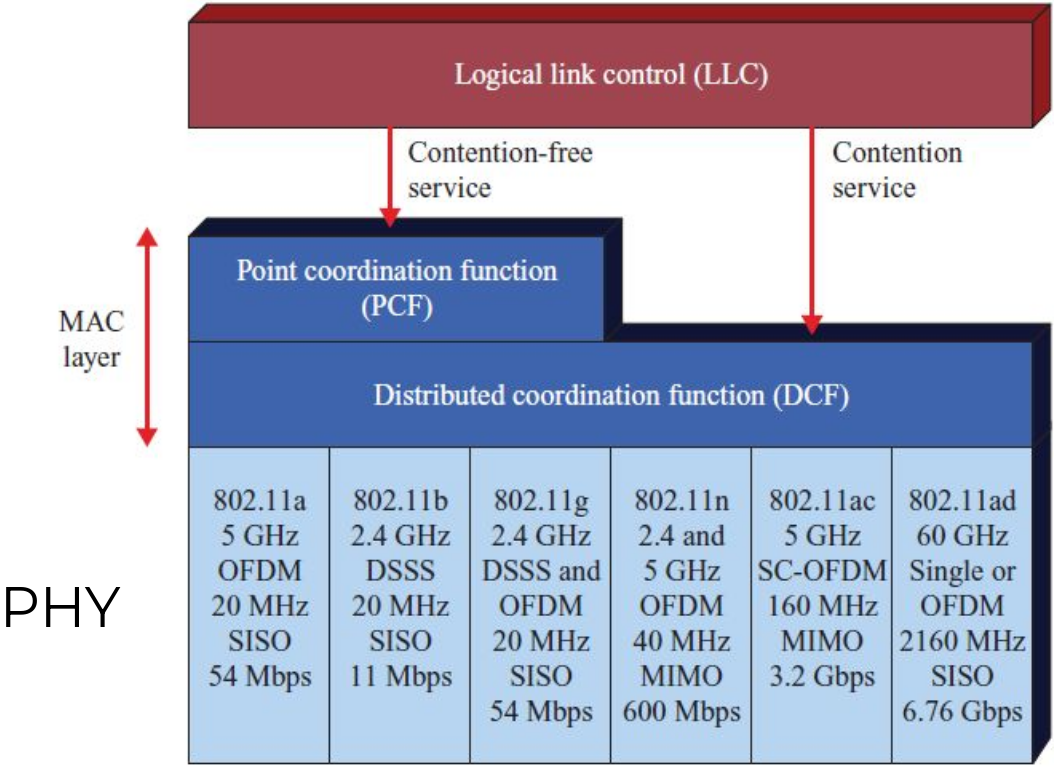
\includegraphics[width=0.75\linewidth]{img/wlan/protarch1}
\end{center}

Mostrate in ordine da sinistra a destra, a livello fisico ci sono le versioni di WiFi, anche se l'ultimo rappresentato non è WiFi 6 (quello è 802.11ax). Sopra c'è il livello MAC, poi il Logical Link Control che permette di avere servizi. 

Il throughput diverso (visibile \href{https://en.wikipedia.org/wiki/IEEE_802.11#Protocol}{\texttt{in questa tabella}}) è determinato da: dimensione del canale, aumentata nel tempo, frequenze utilizzate, modulazioni con più bit per symbol e MIMO (Multiple Input Multiple Output, fino a 16 antenne diverse per fare input/output).

\paragraph{Servizi Logical Link Control LLC:} Offre principalmente tre servizi: 
\begin{itemize}
	\item \textbf{Unacknowledged connectionless service}: consegna non garantita, datagram indipendenti, senza controllo di errori o di flusso; cosa capita capita

	\item \textbf{Connection-mode service}: canale punto-punto, correzione degli errori e controllo di flusso; connessione affidabile

	\item \textbf{Acknowledged connectionless}: datagram indipendent, acknowledged datagram; senza connessione, ma con ack
\end{itemize}

\paragraph{Infrastruttura 802.11:} 
\begin{center}
	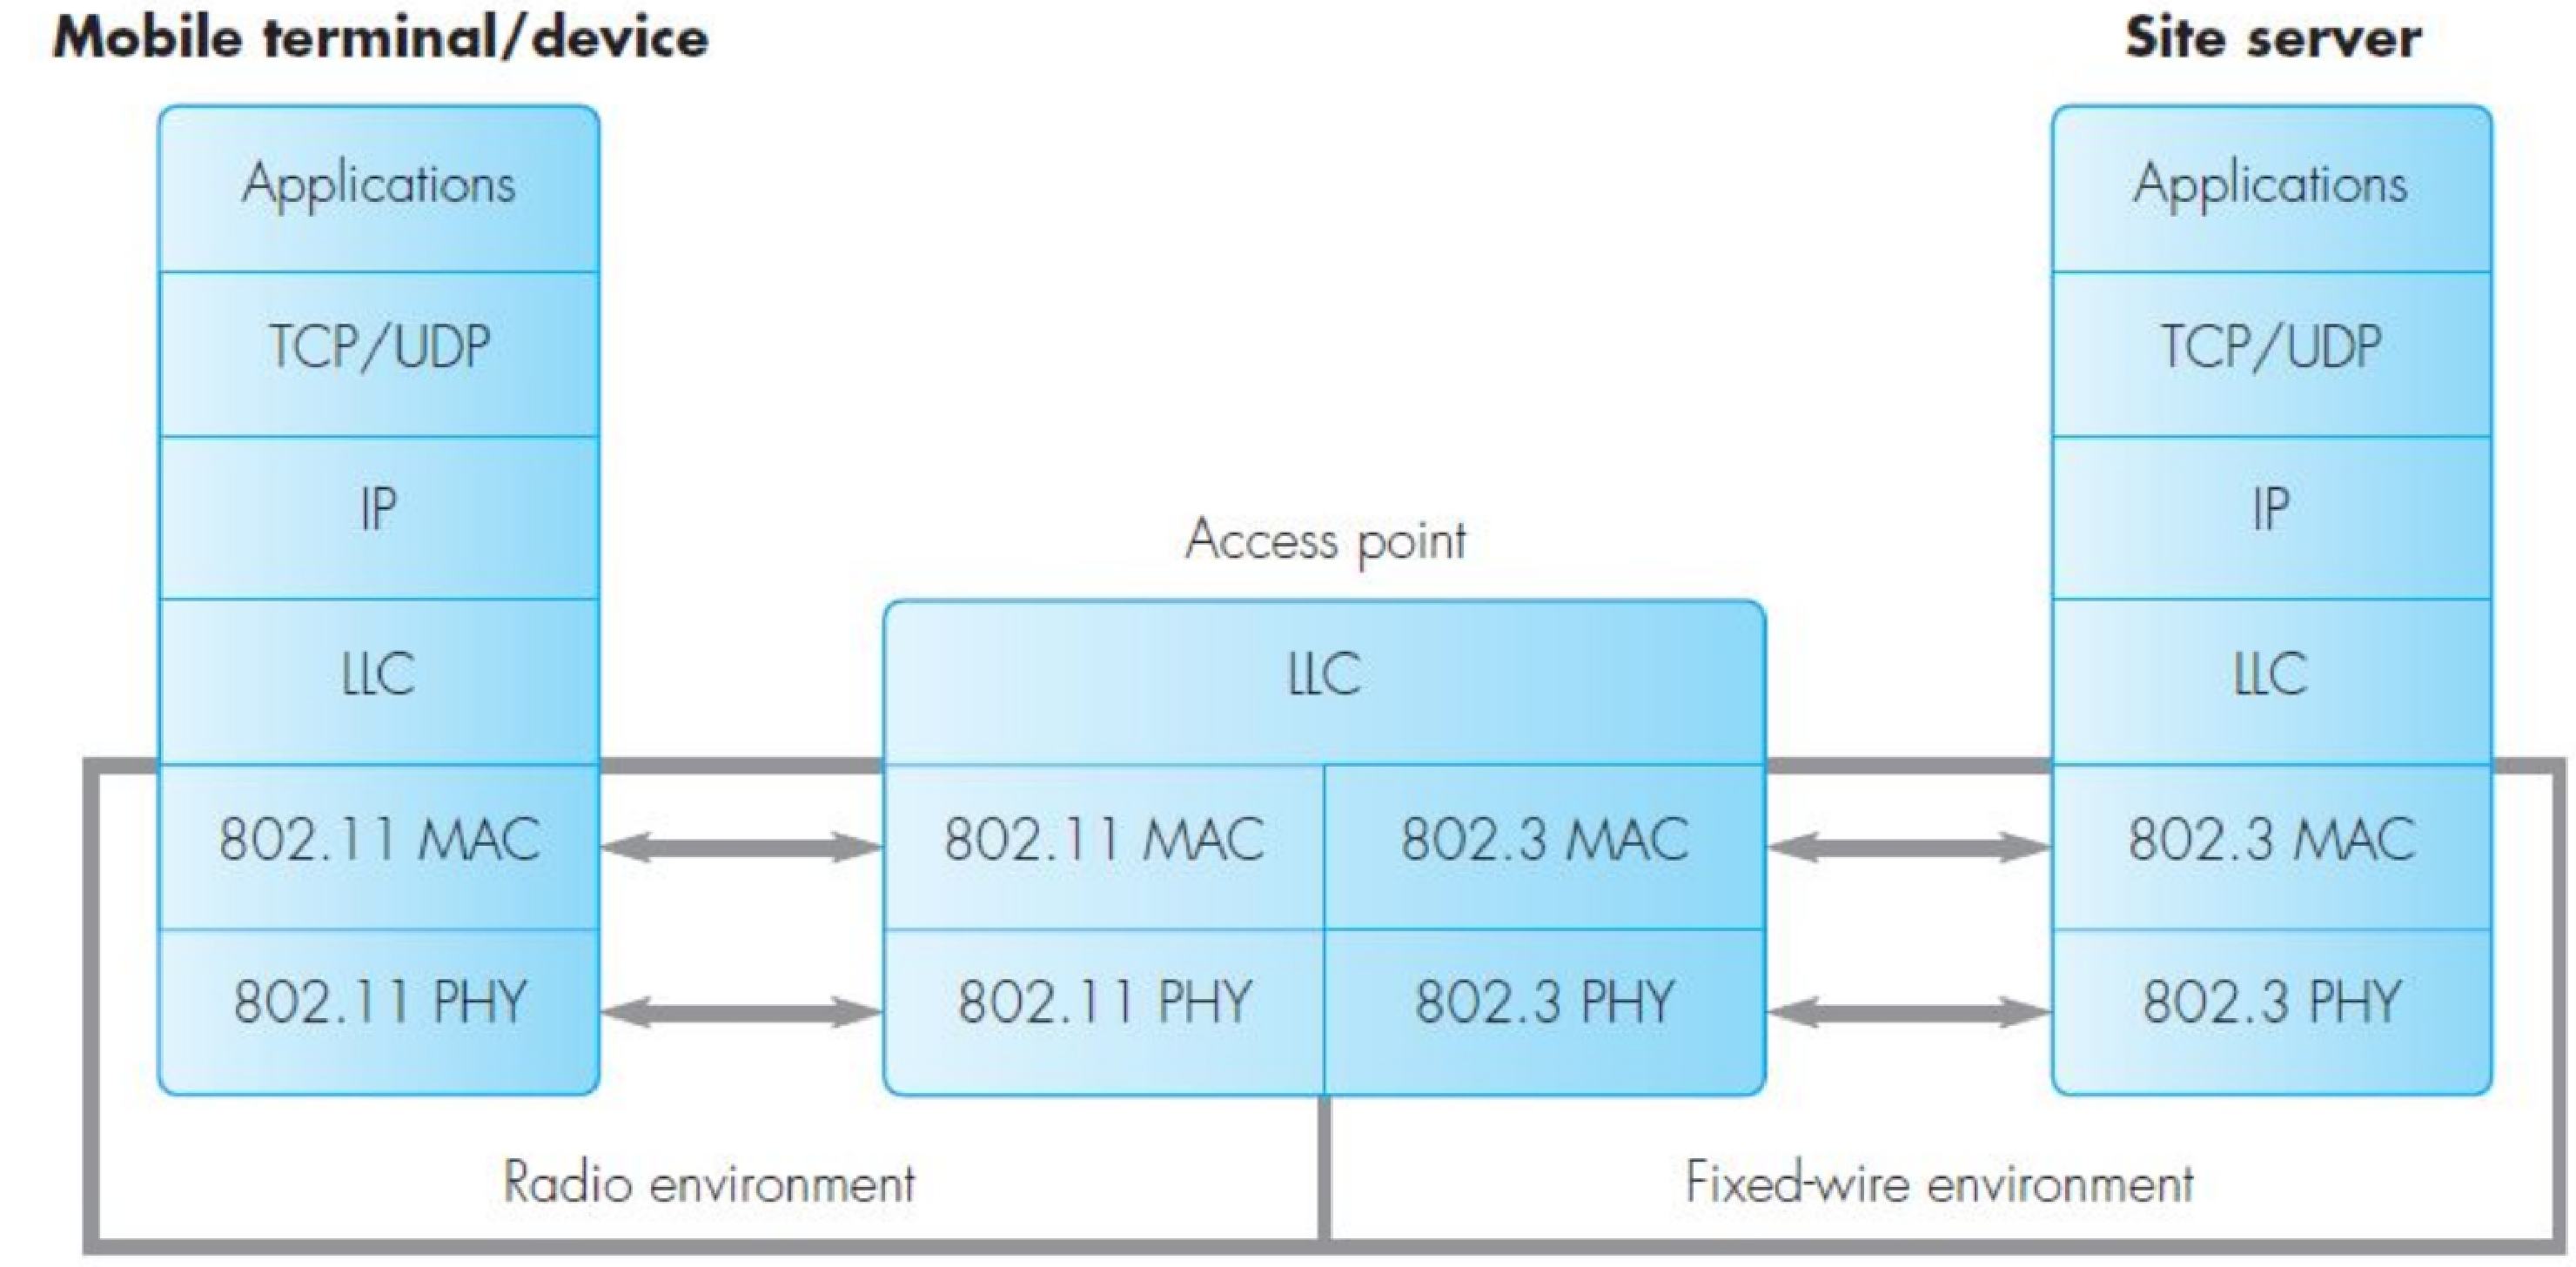
\includegraphics[width=0.85\linewidth]{img/wlan/infr}
\end{center}
Il livello LLC è comune a 802.X.  

\paragraph{Livelli Pacchetti:} La struttura per l'incapsulamento dei livelli è 
\begin{center}
	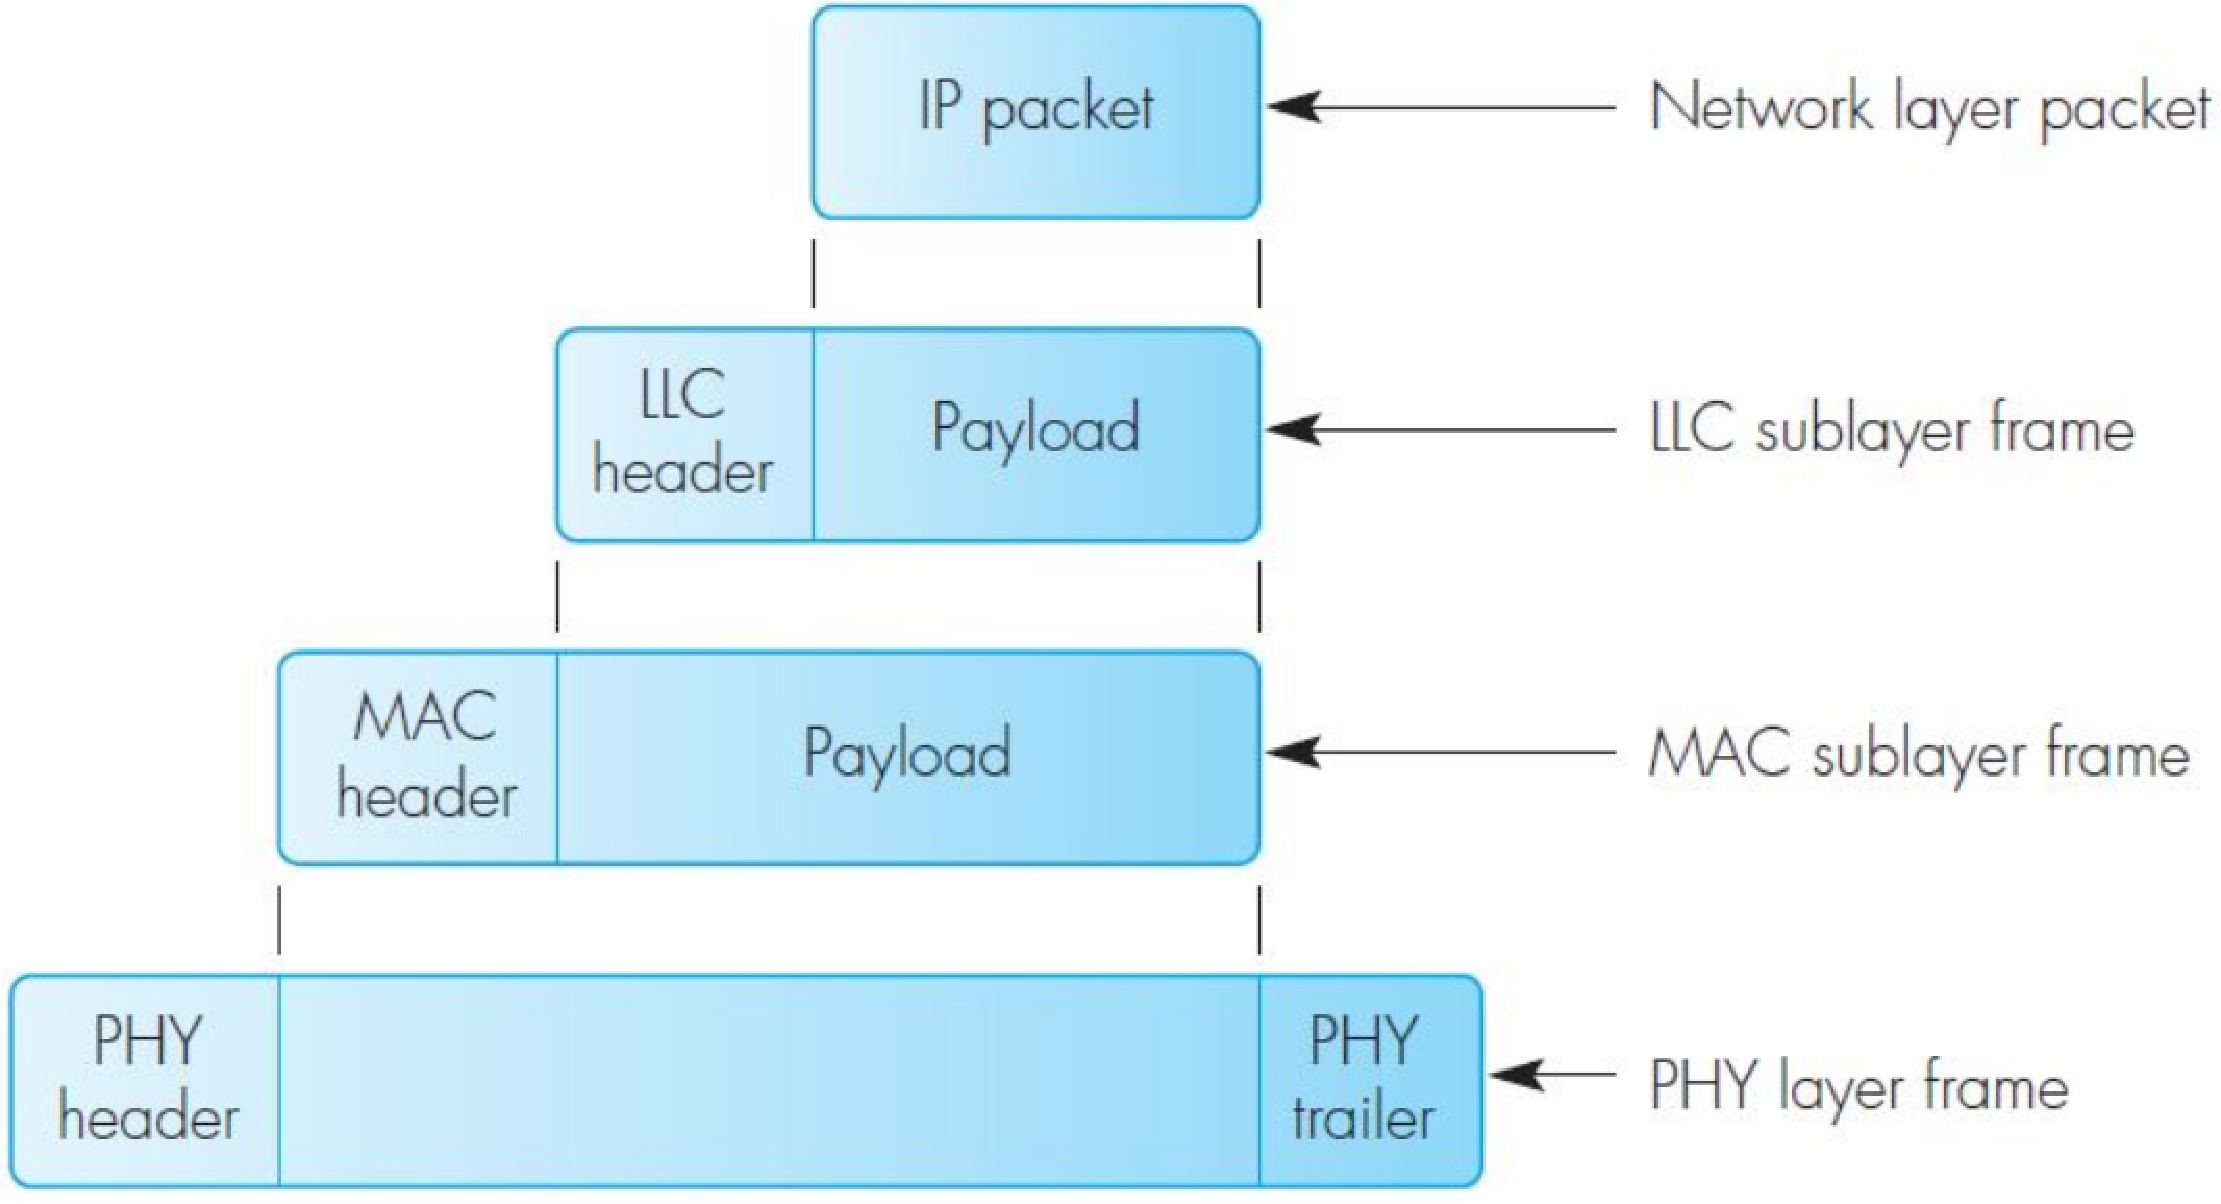
\includegraphics[width=0.6\linewidth]{img/wlan/pacch1}
\end{center}
Ovvero, fisico, MAC, LLC, poi pacchetto di rete.

\subsection{802.11 Senza Infrastruttura}

Si ha un canale \textit{molto} inaffidabile (rispetto a uno cablato), con molte informazioni da trasmettere, e di conseguenza frame più complessi (rispetto a 802.3). Il frame di MAC 802.11 ha un payload massimo di $2304B$.

Il \textbf{sottolivello MAC} offre due servizi: 
\begin{itemize}
	\item Servizio \textbf{dati asincrono}: non ha garanzie sul delay e quindi sulla QoS, best effort
	
    \item Servizio \textbf{time-bounded}: offre garanzie sul delay, disponibile solo in presenza di un coordinatore (AP)
\end{itemize}

\subsubsection{Distributed Coordination Function DCF}

Opera in \textbf{CSMA/CA}: l'accesso al canale deve essere regolato aspettando \textit{del tempo} prima di poter trasmettere. 802.11 prevede diversi tempi di attesa a seconda della tipologia di dati da trasmettere.

Definizioni:
\begin{itemize}
	\item \textbf{Slot time}: una unità base di tempo (interna al dispositivo), non si tratta di una suddivisione temporale; tiene conto del ritardo di propagazione e della tipologia di trasmettitore utilizzato (tipo di WiFi fisico usato, es: 20$\mu s$ per 802.11b)

	\item \textbf{Short Inter-frame Spacing SIFS}: l'intervallo più breve di attesa usato per messaggi ad alta priorità, altra unità base di tempo; la durata dipende dalla tipologia di trasmettitore

	\item \textbf{DCF Inter-frame Spacing DIFS}: intervallo di tempo più lungo usato per messaggi a bassa priorità best effort: \texttt{SIFS+ 2*slot\_time}

	\item \textbf{PCF Inter-frame Spacing PIFS}: intervallo di tempo intermedio per time-bounded: \texttt{SIFS+1*slot\_time}
\end{itemize}

Nel caso di \textbf{trasmissione con canale libero}:
\begin{itemize}
	\item il sender inizia ad ascoltare il canale
	
    \item fa un Clear Channel Assessment CCA
	
    \item ascolta per un tempo \textit{lungo} (ovvero DIFS) il canale
	
    \item fa un altro CCA
\end{itemize}

Se il canale è risultato libero durante entrambi CCA allora il dispositivo può cominciare a trasmettere.

Se \textbf{non è necessario ack}, una volta terminata la trasmissione il canale è libero.

Se \textbf{necessario l'ack}, l'attesa dell'acknowledgement ha durata \textit{breve} SIFS (più breve del tempo per i CCA, altrimenti potrebbe andare in conflitto con CCA di altri dispositivi); dal RX l'ack viene inviato il prima possibile (giusto il tempo di turnaround e di preparare il pacchetto).

Se il \textbf{frame viene corrotto} prima della ricezione, mancherà l'ack: il TX aspetta tempo SIFS e, se non riceve niente, assume che la trasmissione non sia andata a buon fine, di conseguenza ritrasmette subito lo stesso frame; "subito" perché ha ottenuto l'accesso esclusivo al canale e questo viene tenuto finché la trasmissione non è terminata; il tempo è breve per evitare che altri "si intromettano". Il rilascio del canale avviene solo a trasmissione completata e ack ricevuto. Da standard 802.11 è previsto un massimo di tentativi.
\begin{center}
	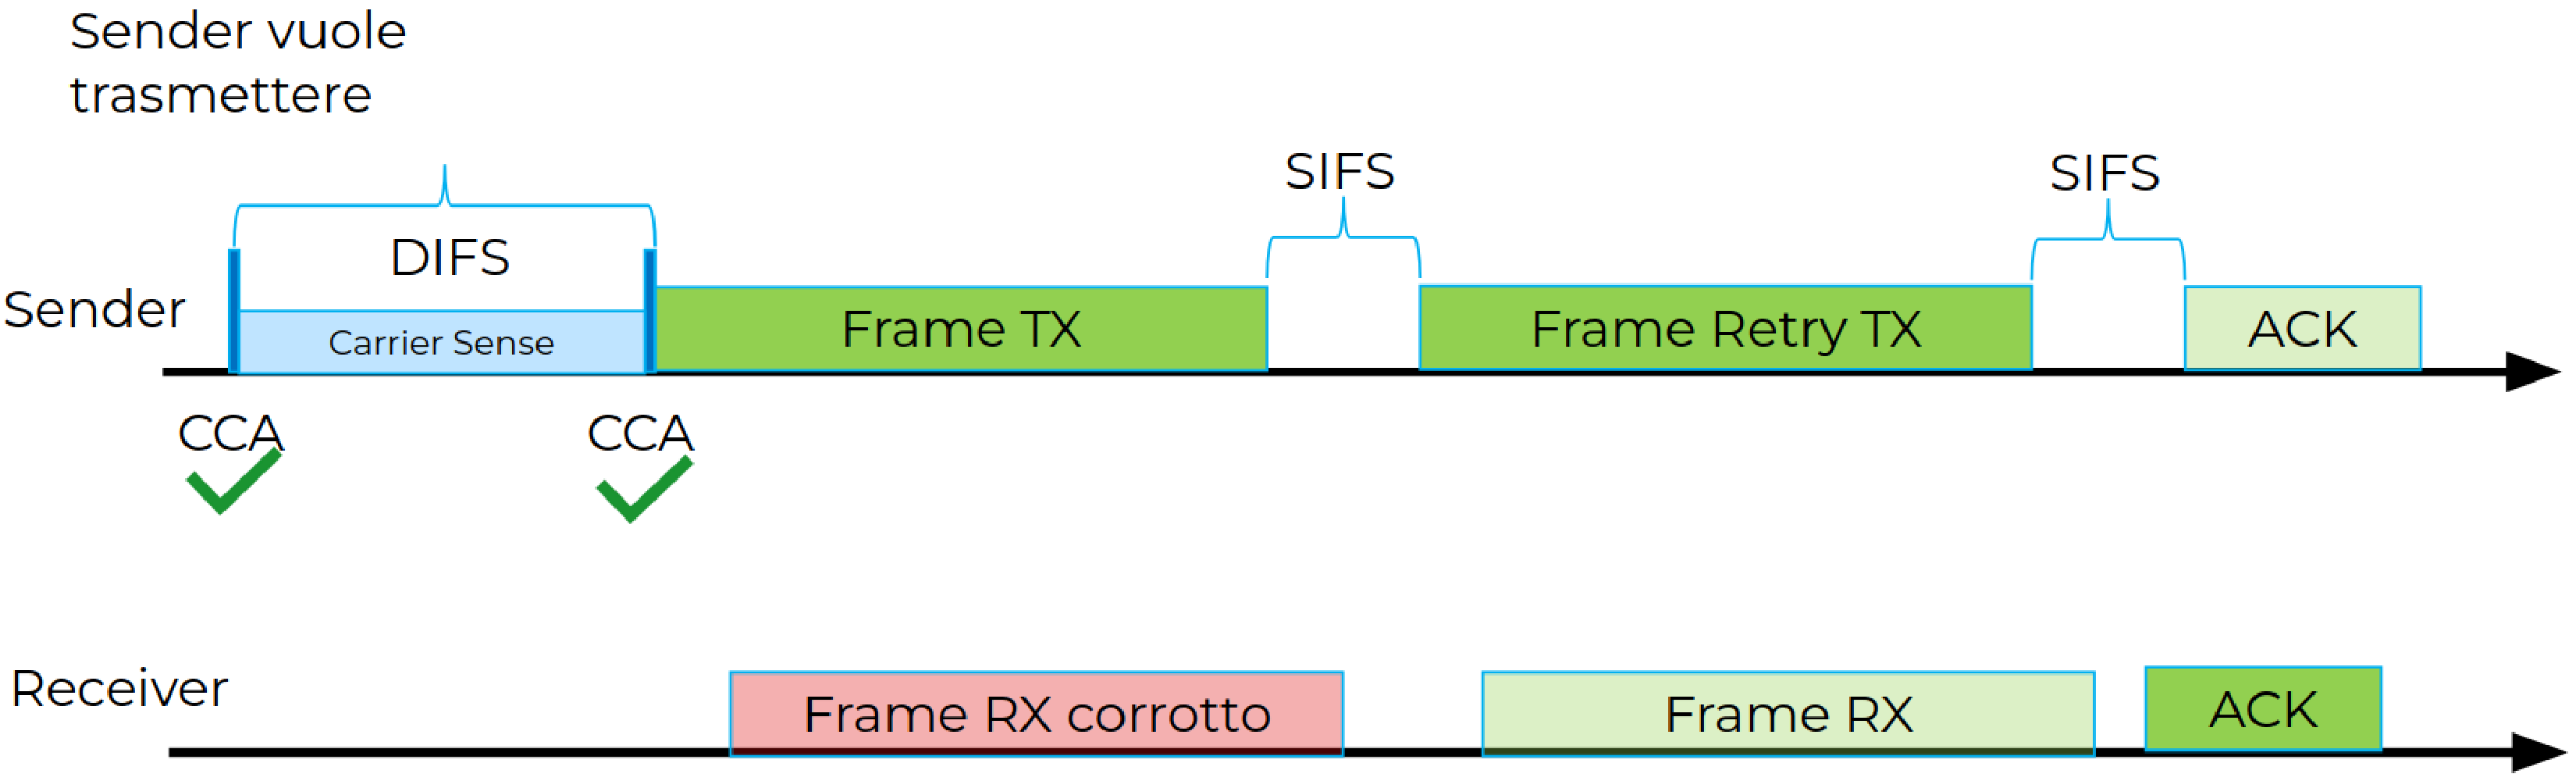
\includegraphics[width=0.98\linewidth]{img/wlan/dcfcsmaca}
\end{center}

Se il \textbf{canale è occupato}, ovvero durante il tempo di attesa DIFS viene ricevuto un segnale, fallisce il CCA ed il dispositivo ascolta fino al termine della trasmissione dell'altro sender.

Quando il canale è di nuovo libero (nuovo CCA), si aspetta un periodo di tempo DIFS, PIFS o SIFS, deciso in base alla priorità del messaggio, prima di avere un periodo di contesa (tutti i dispositivi che devono trasmettere aspettano il momento di fine trasmissione). Durante il periodo di contesa il dispositivo aspetta un numero random di \texttt{slot\_time} da attendere (Binary Exponential Backoff). Viene fatta carrier sense durante tutto il periodo di backoff.
\begin{center}
	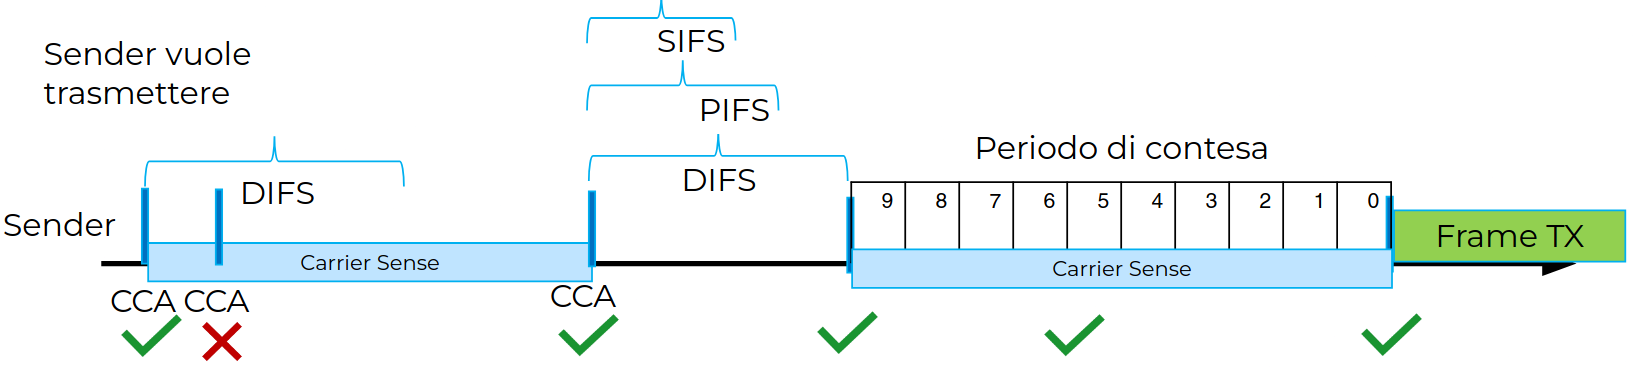
\includegraphics[width=0.98\linewidth]{img/wlan/occupied1}
\end{center}

Da notare come la radio rimanga sempre accesa, non ci sono più requisiti di batteria come in Bluetooth o ZigBee.

Se durante il periodo di contesa il \textbf{canale diventa occupato}, due opzioni:
\begin{enumerate}
	\item Riparto dalla contesa (con intervallo più ampio) al prossimo ciclo; non equa nei confronti delle stazioni che hanno "perso", rischio attesa infinita
    
	\item Blocco il timer al valore in cui era arrivato nel momento in cui è stato rilevato il canale occupato e nel \textbf{turno successivo riparto} da quel valore
\end{enumerate}

\subsubsection{Problema del terminale nascosto}

Il meccanismo di carrier sense funziona se l'altro dispositivo che comincia a trasmettere può essere rilevato. Ad esempio, nel caso
\begin{center}
	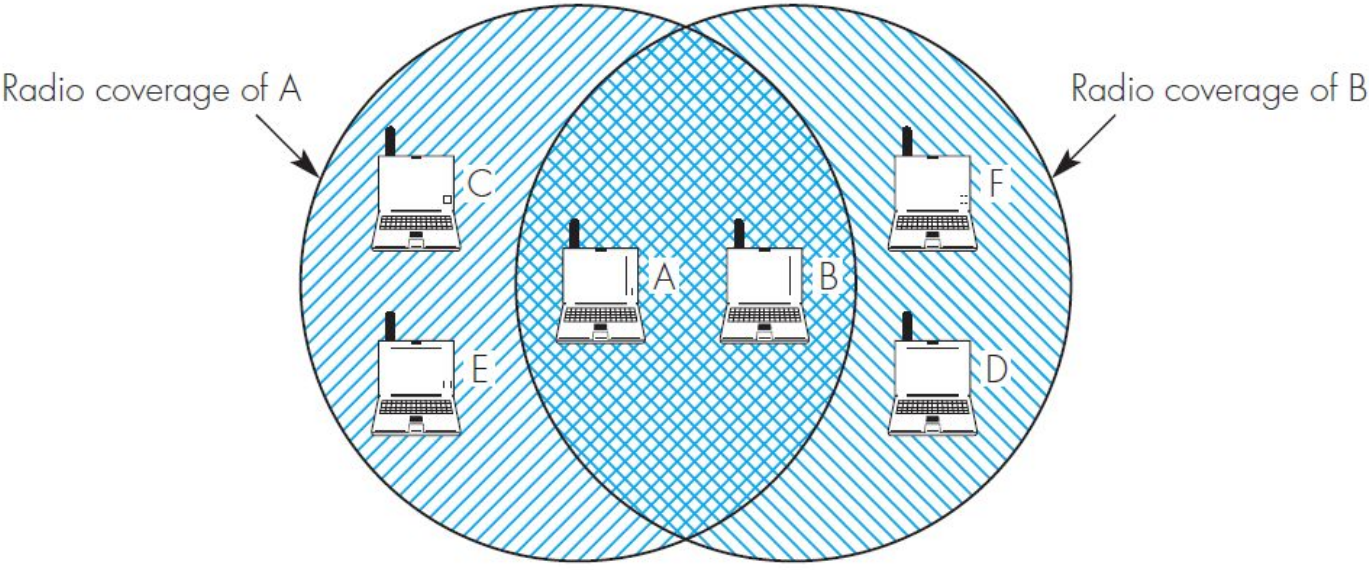
\includegraphics[width=0.8\linewidth]{img/wlan/sneaky}
\end{center}

A e D non si possono "sentire" a vicenda, in quanto fuori dal rispettivo raggio di copertura. Se entrambi volessero trasmettere a B vedrebbero il canale libero nello stesso momento, causando una collisione.
\begin{center}
	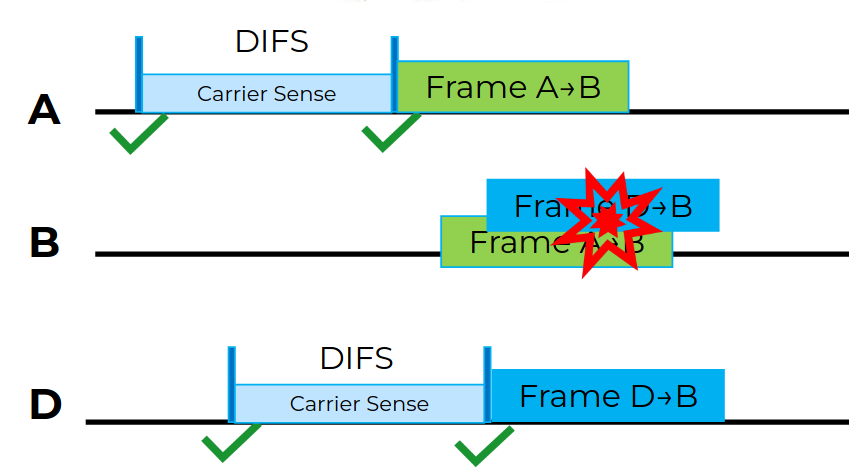
\includegraphics[width=0.65\linewidth]{img/wlan/boom}
\end{center}

Per risolvere, dopo aver fatto carrier sense, il sender invia una \textbf{Request to Send RTS} contenente sorgente e destinazione della richiesta oltre alla durata stimata da RTS ad ack finale.

Il RTS viene ricevuto da tutti i terminali nel raggio di copertura del sender, i quali sanno che la richiesta non è per loro e usano le informazioni sul tempo previsto per allocare un \textbf{Network Allocation Vector NAV}, ovvero un tempo nella quale sanno che non potranno trasmettere.

Il destinatario, se è libero, risponderà (dopo tempo SIFS, per evitare che comincino altre comunicazioni nel frattempo) con un \textbf{Clear to Send CTS}, contenente sorgente, destinazione e il tempo rimanente fino alla fine della trasmissione (stima precedente meno il tempo passato).

Il CTS viene ricevuto da tutti i terminali nel raggio del destinatario, i quali allocheranno un \textbf{NAV} per il tempo indicato nel CTS (ovviamente minore di quello del RTS). In questo modo vengono a conoscenza del fatto che un altro nodo all'esterno del loro raggio di copertura vuole comunicare con un nodo a loro visibile, quindi non tentano nemmeno di accedere al canale.

Dopo che il sender originale ha ricevuto il CTS aspetta SIFS per poi inviare il frame e aspettare di ricevere l'ack per terminare la trasmissione.
\begin{center}
	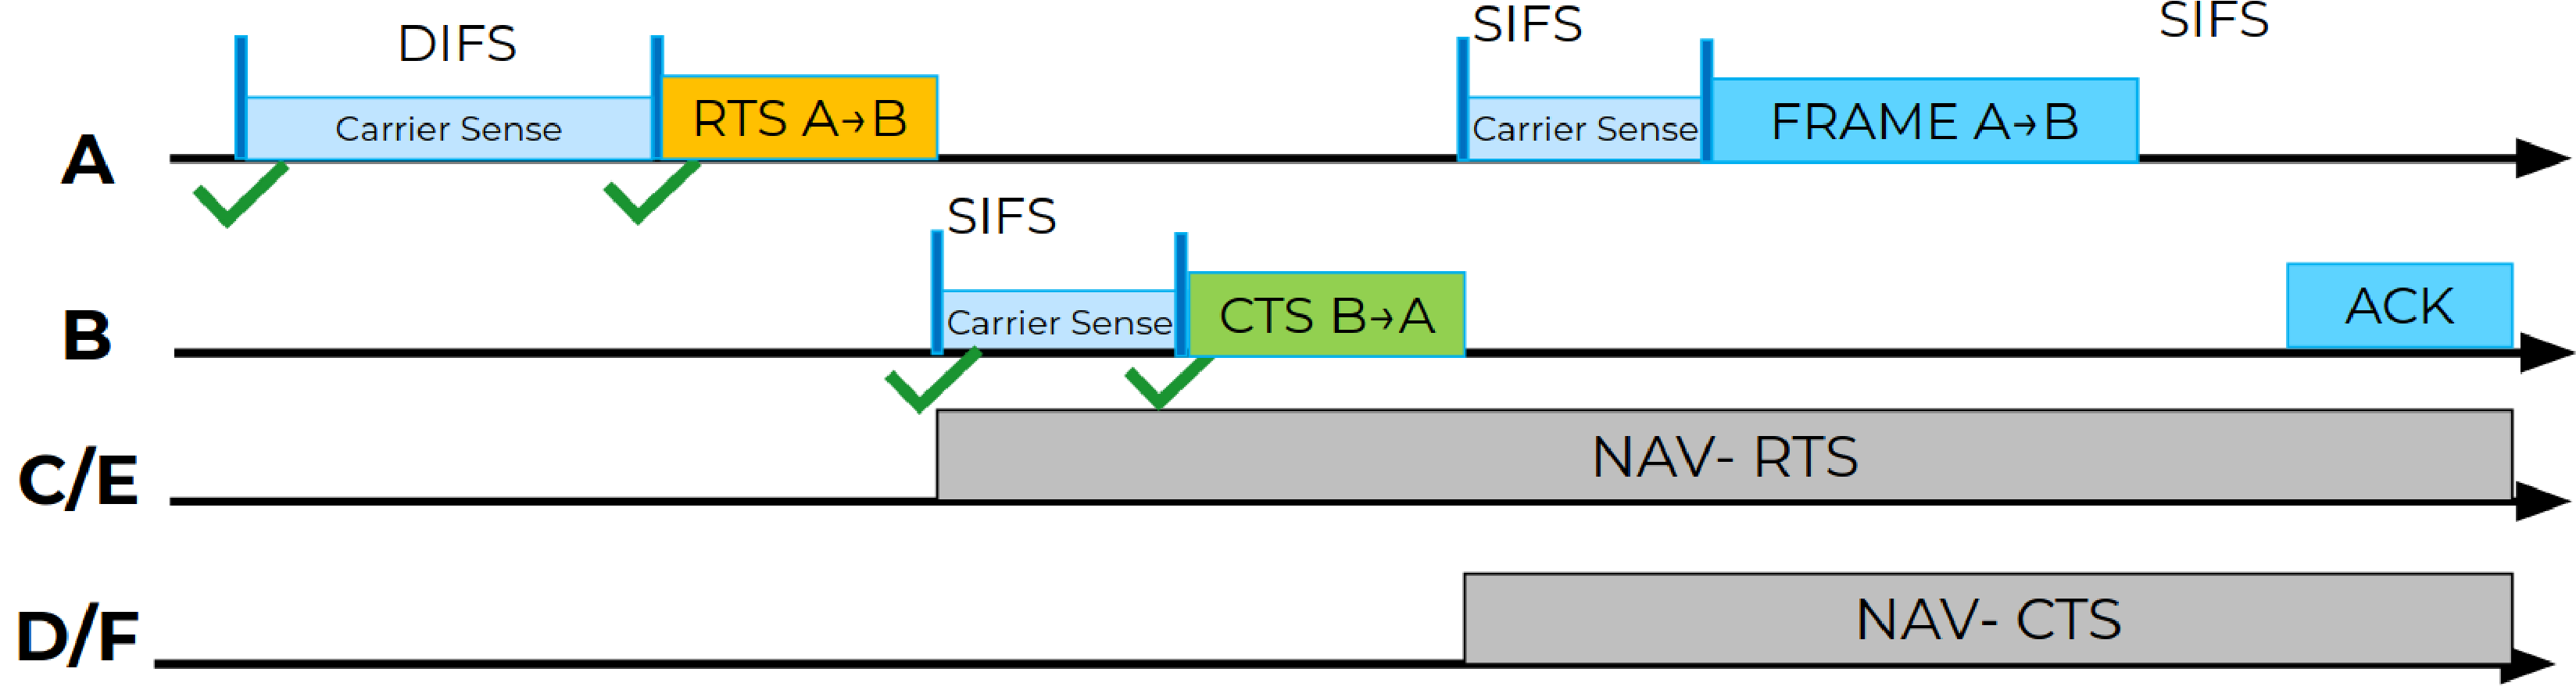
\includegraphics[width=0.99\linewidth]{img/wlan/rtscts}
\end{center}

\paragraph{Frammentazione:} Il canale radio è molto più sensibile ad interferenza e rumore. Considerando la dimensione della frame Ethernet (1522 byte) è molto probabile che ogni frame abbia errori; meglio \textbf{ridurre la dimensione della frame MAC}. 

Una Frame LLC viene suddivisa in frammenti più piccoli la cui dimensione è variabile in base alle condizioni del canale.
\begin{center}
	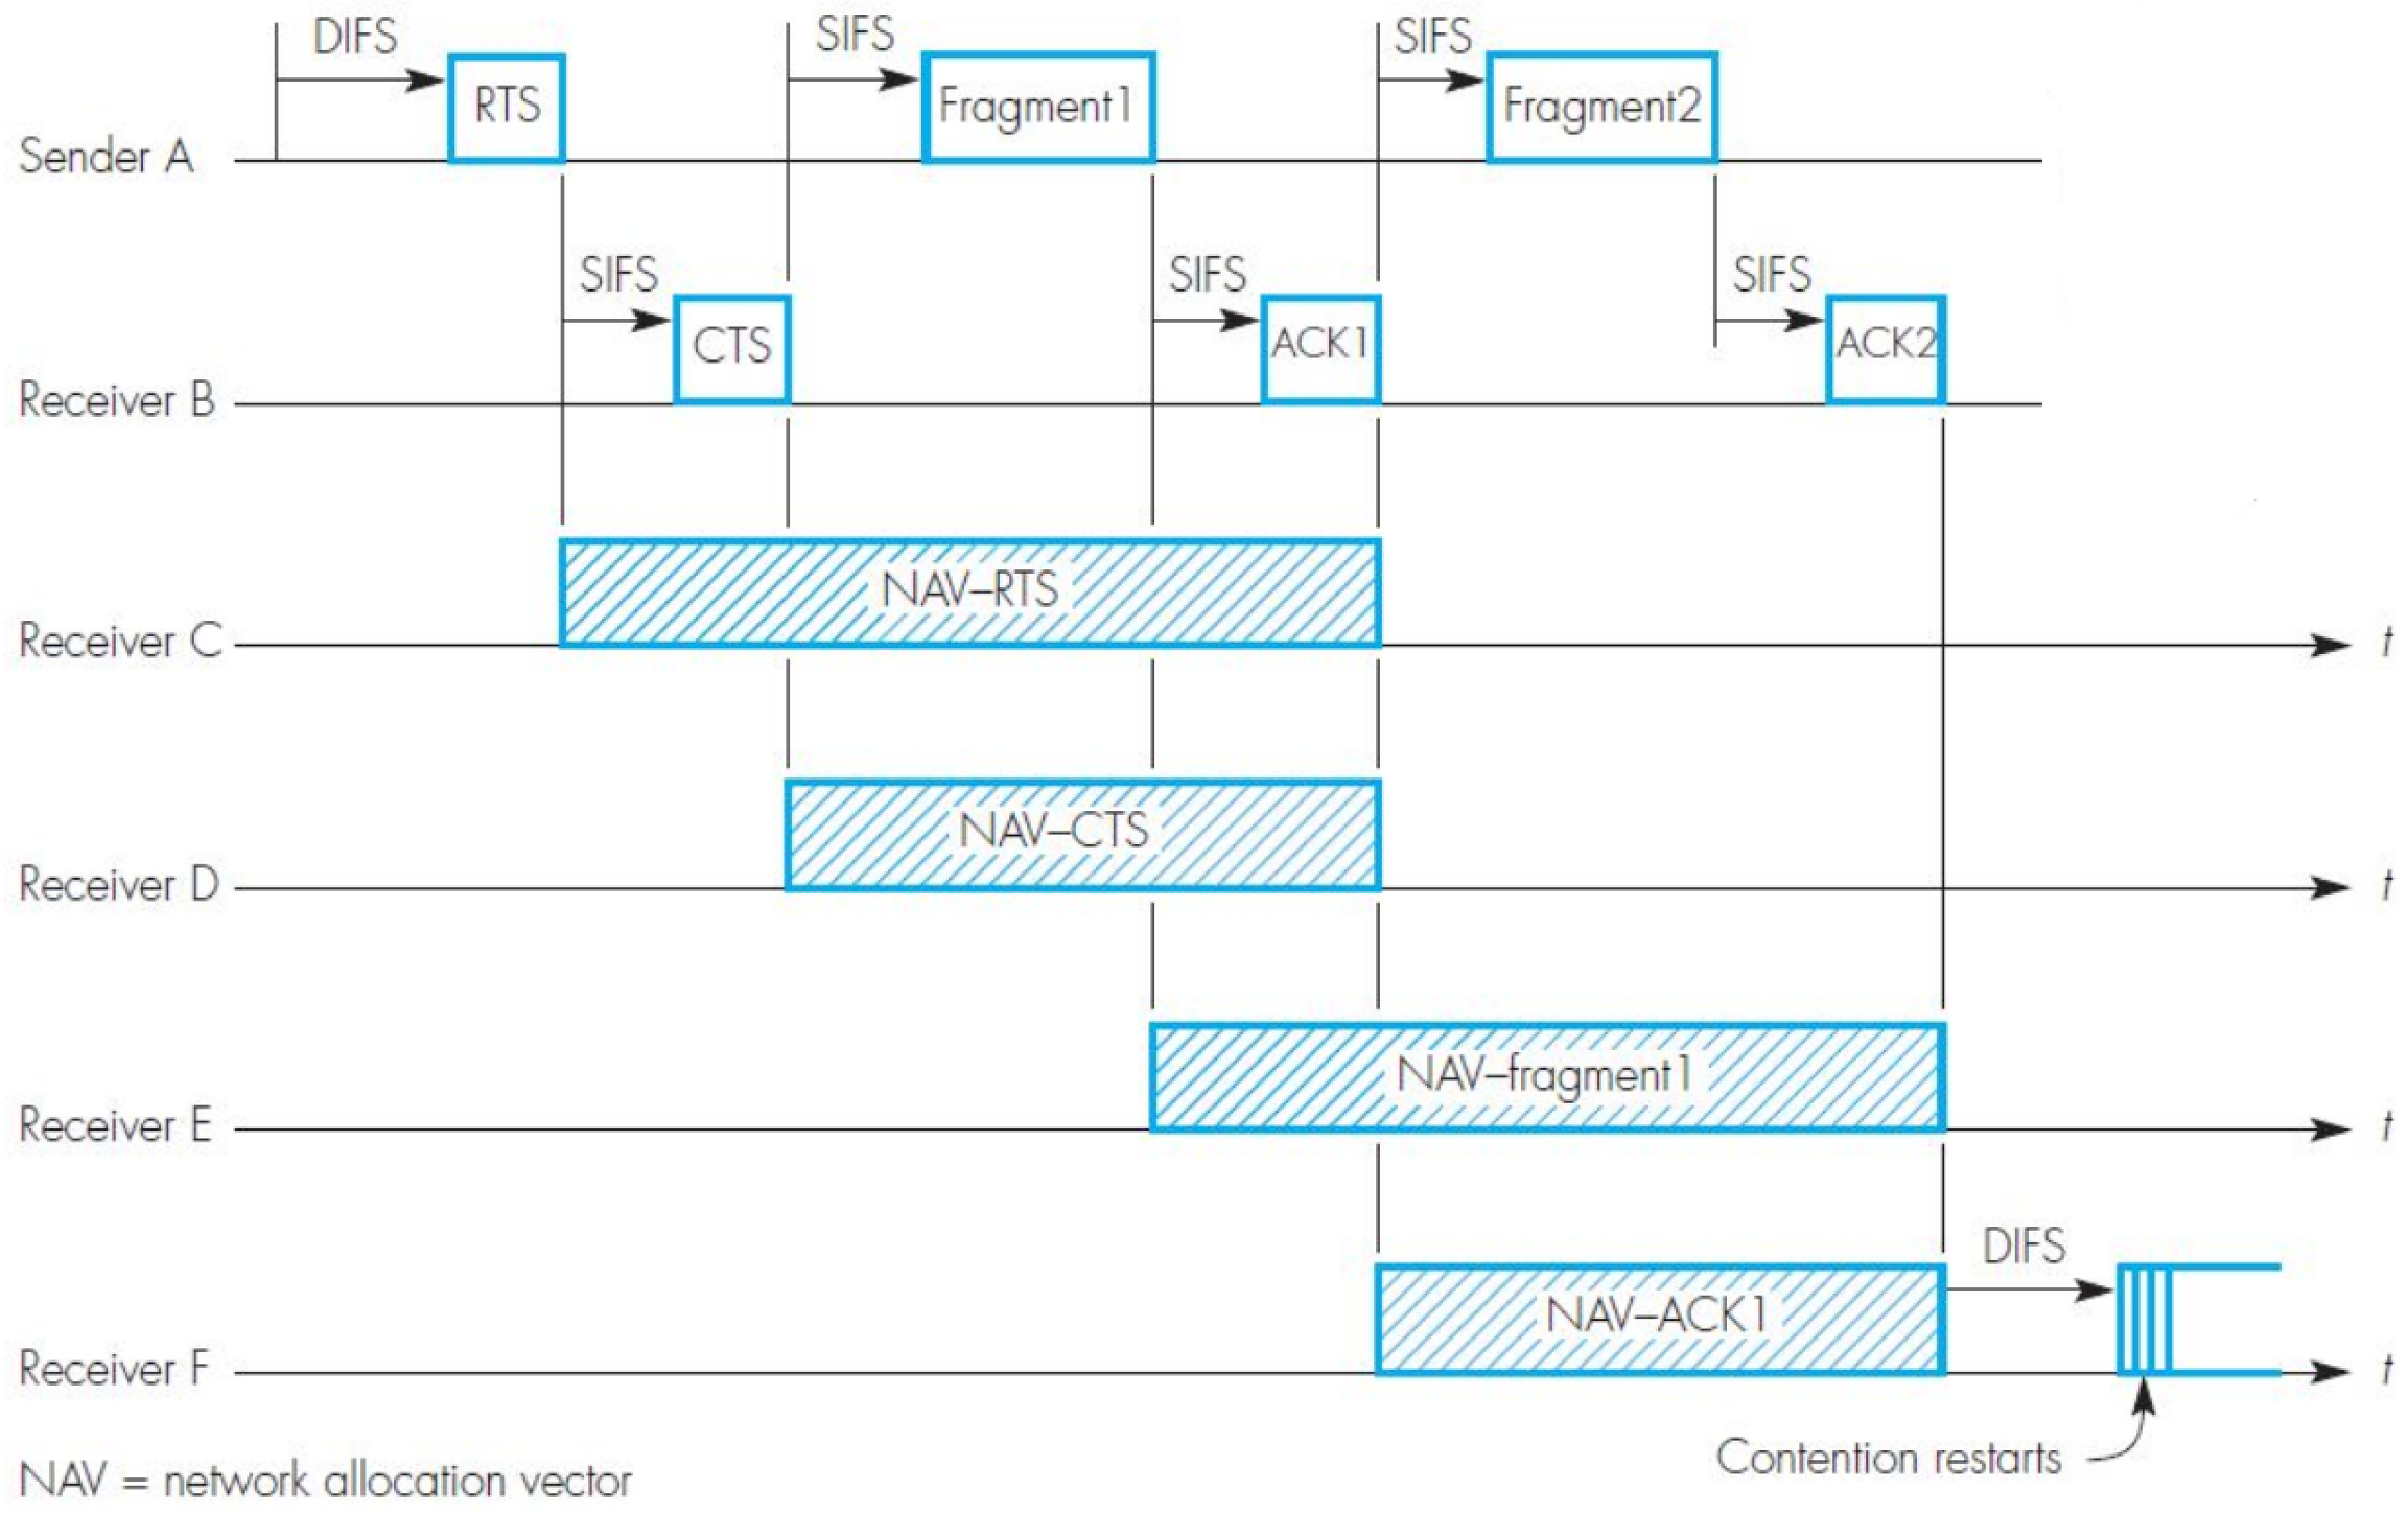
\includegraphics[width=0.9\linewidth]{img/wlan/frag}
\end{center}

All'interno di ogni "frammento" si inseriscono informazioni riguardo al NAV per i dispositivi non direttamente coinvolti nella comunicazione.

La frammentazione e correzione dei dati viene fatta a livello MAC, tra dispositivo e AP, dove il ritardo dovuto alla correzione è minimo. Si potrebbe lasciare la correzione dei dati al livello superiore (TCP), ma sarebbe il destinatario finale e non l'AP ad accorgersi dell'errore, allungando di molto i tempi di ritrasmissione (la ritrasmissione deve arrivare prima alla destinazione finale per poi tornare indietro, mentre l'AP è il primo hop).

\subsection{802.11 Con Infrastruttura}

Nel caso più semplice si ha un solo AP con il relativo Basic Service Set BSS, l'insieme di stazioni controllate dal singolo coordinatore. Si può anche avere un Extended Service Set ESS, ovvero un insieme di più BSS interconnessi tramite un sistema distribuito (DS).
\begin{center}
	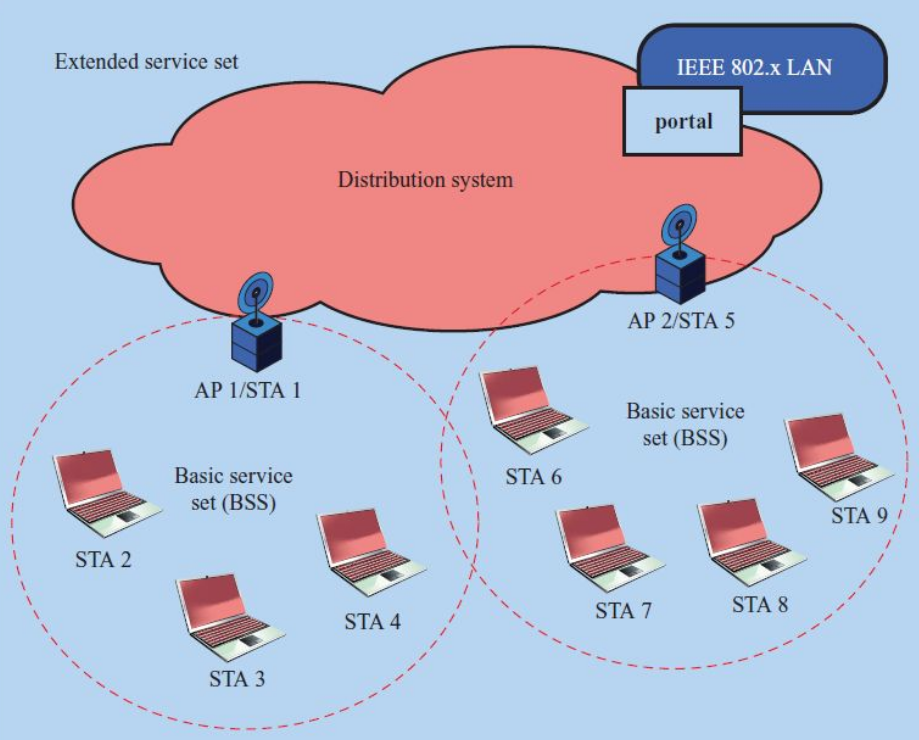
\includegraphics[width=0.8\linewidth]{img/wlan/ess}
\end{center}

Con "portale" si intende un router/bridge che collega il sistema distribuito alla LAN. ESS viene visto come un unico BSS a livello LLC per funzionalità di roaming (muovermi nella rete e rimanere collegato) tra AP diversi (overlapping almeno 10\% per garantire continuità).

\subsubsection{Point Coordination Function}

In presenza di un AP, tutti i frame passano per quest'ultimo. Questo permette di avere \textbf{servizi time-bounded}, con garanzie sul delay, non possibili con DCF (il random backoff non fornisce garanzie). Nella modalità PCF, l'AP controlla l'accesso al canale radio: 
\begin{enumerate}
	\item Tutto il traffico passa dall'AP
    
	\item Le stazioni associate ad AP usano DCF con tempistiche SIFS e DIFS per accedere al canale

	\item AP usa PIFS
\end{enumerate}
In questo modo AP riesce ad "impossessarsi" del canale radio prima delle stazioni in attesa.

AP manda messaggi periodici ($10$-$100s$) detti \textbf{beacon frame} che sono frame di gestione contenenti
\begin{enumerate}
	\item Parametri operativi PHY (bit rate \& Modulation Coding Scheme)

	\item Sincronizzazione (usato nelle prime versioni 802.11 che usavano FHSS)

	\item Supporto a PCF con le relative informazioni

	\item Invito per le nuove stazioni che non sono ancora associate
\end{enumerate}
Ovvero, una rete manda dei beacon per "farsi scoprire" e comunicare le proprie caratteristiche per le nuove associazioni.

Il tempo è diviso in blocchi (superframe), all'interno dei quali si ha una divisione in due periodi:
\begin{itemize}
	\item una parte \textbf{senza contesa}, opzionale, ma necessaria per servizi time bounded
    
	\item accesso \textbf{a contesa}, sempre presente
\end{itemize}
\begin{center}
	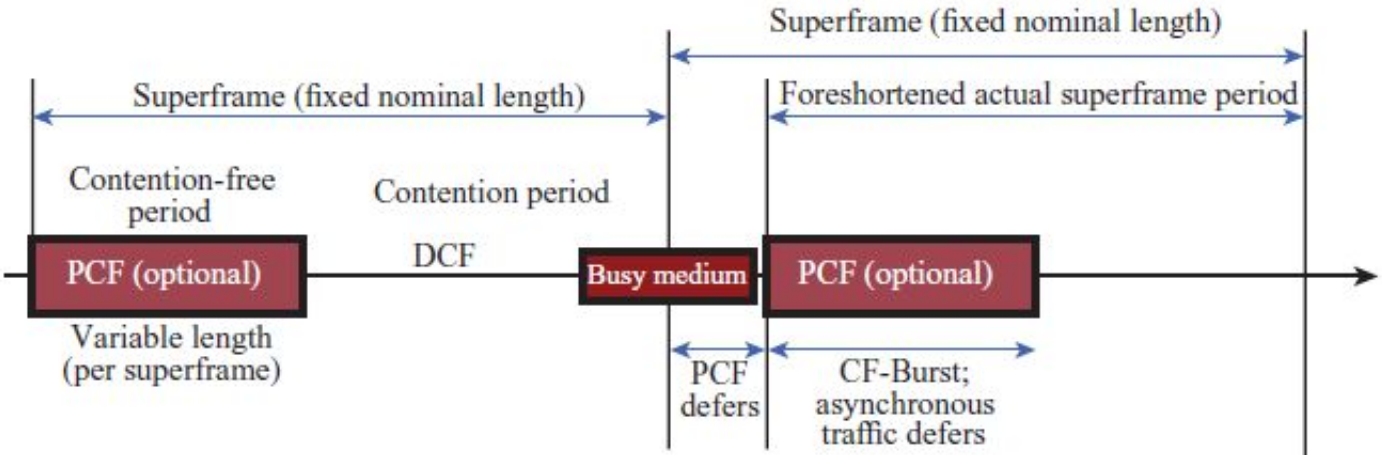
\includegraphics[width=0.95\linewidth]{img/wlan/superframe}
\end{center}

Se il canale radio è occupato oltre il limite del superframe il tempo non verrà recuperato (si aspetta).

Quindi la PCF ha un funzionamento del tipo:
\begin{center}
	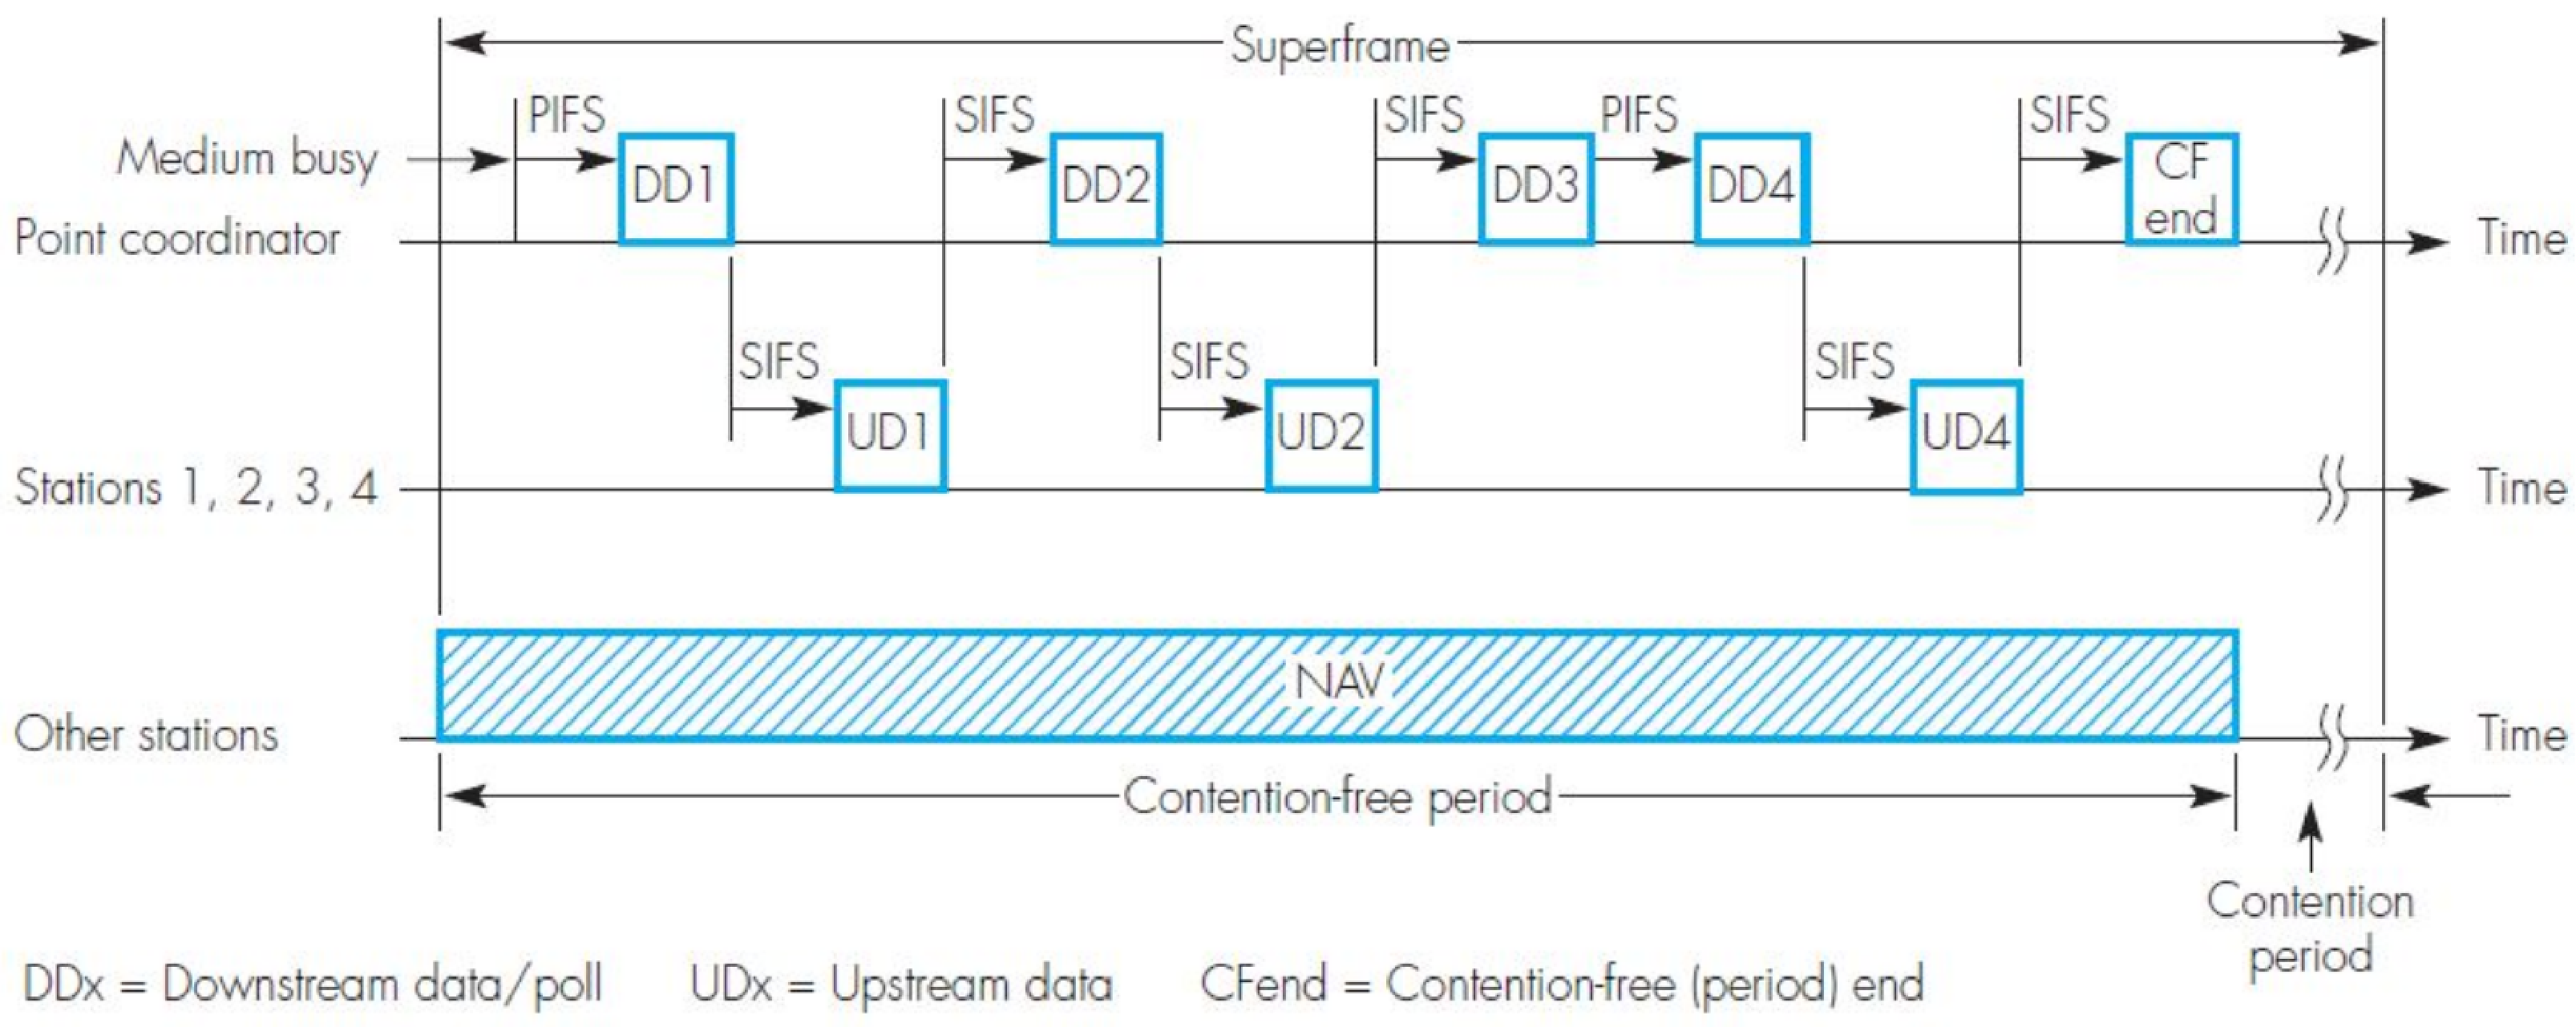
\includegraphics[width=0.98\linewidth]{img/wlan/pcf1}
\end{center}

Al termine della comunicazione precedente, tutti i dispositivi cominciano ad attendere DIFS, ma l'AP aspetta PIFS, quindi prende il lock sul canale prima degli altri, iniziando il periodo senza contesa. 

In seguito l'AP invia il "permesso di trasmettere" per ogni trasmissione necessaria, aspettando SIFS tra una e l'altra (per non rischiare di perdere il lock sul canale). Al termine si manda un Contention Free End per marcare la fine del periodo senza contesa.

% End L10

\subsubsection{Formato Frame MAC}
\begin{center}
	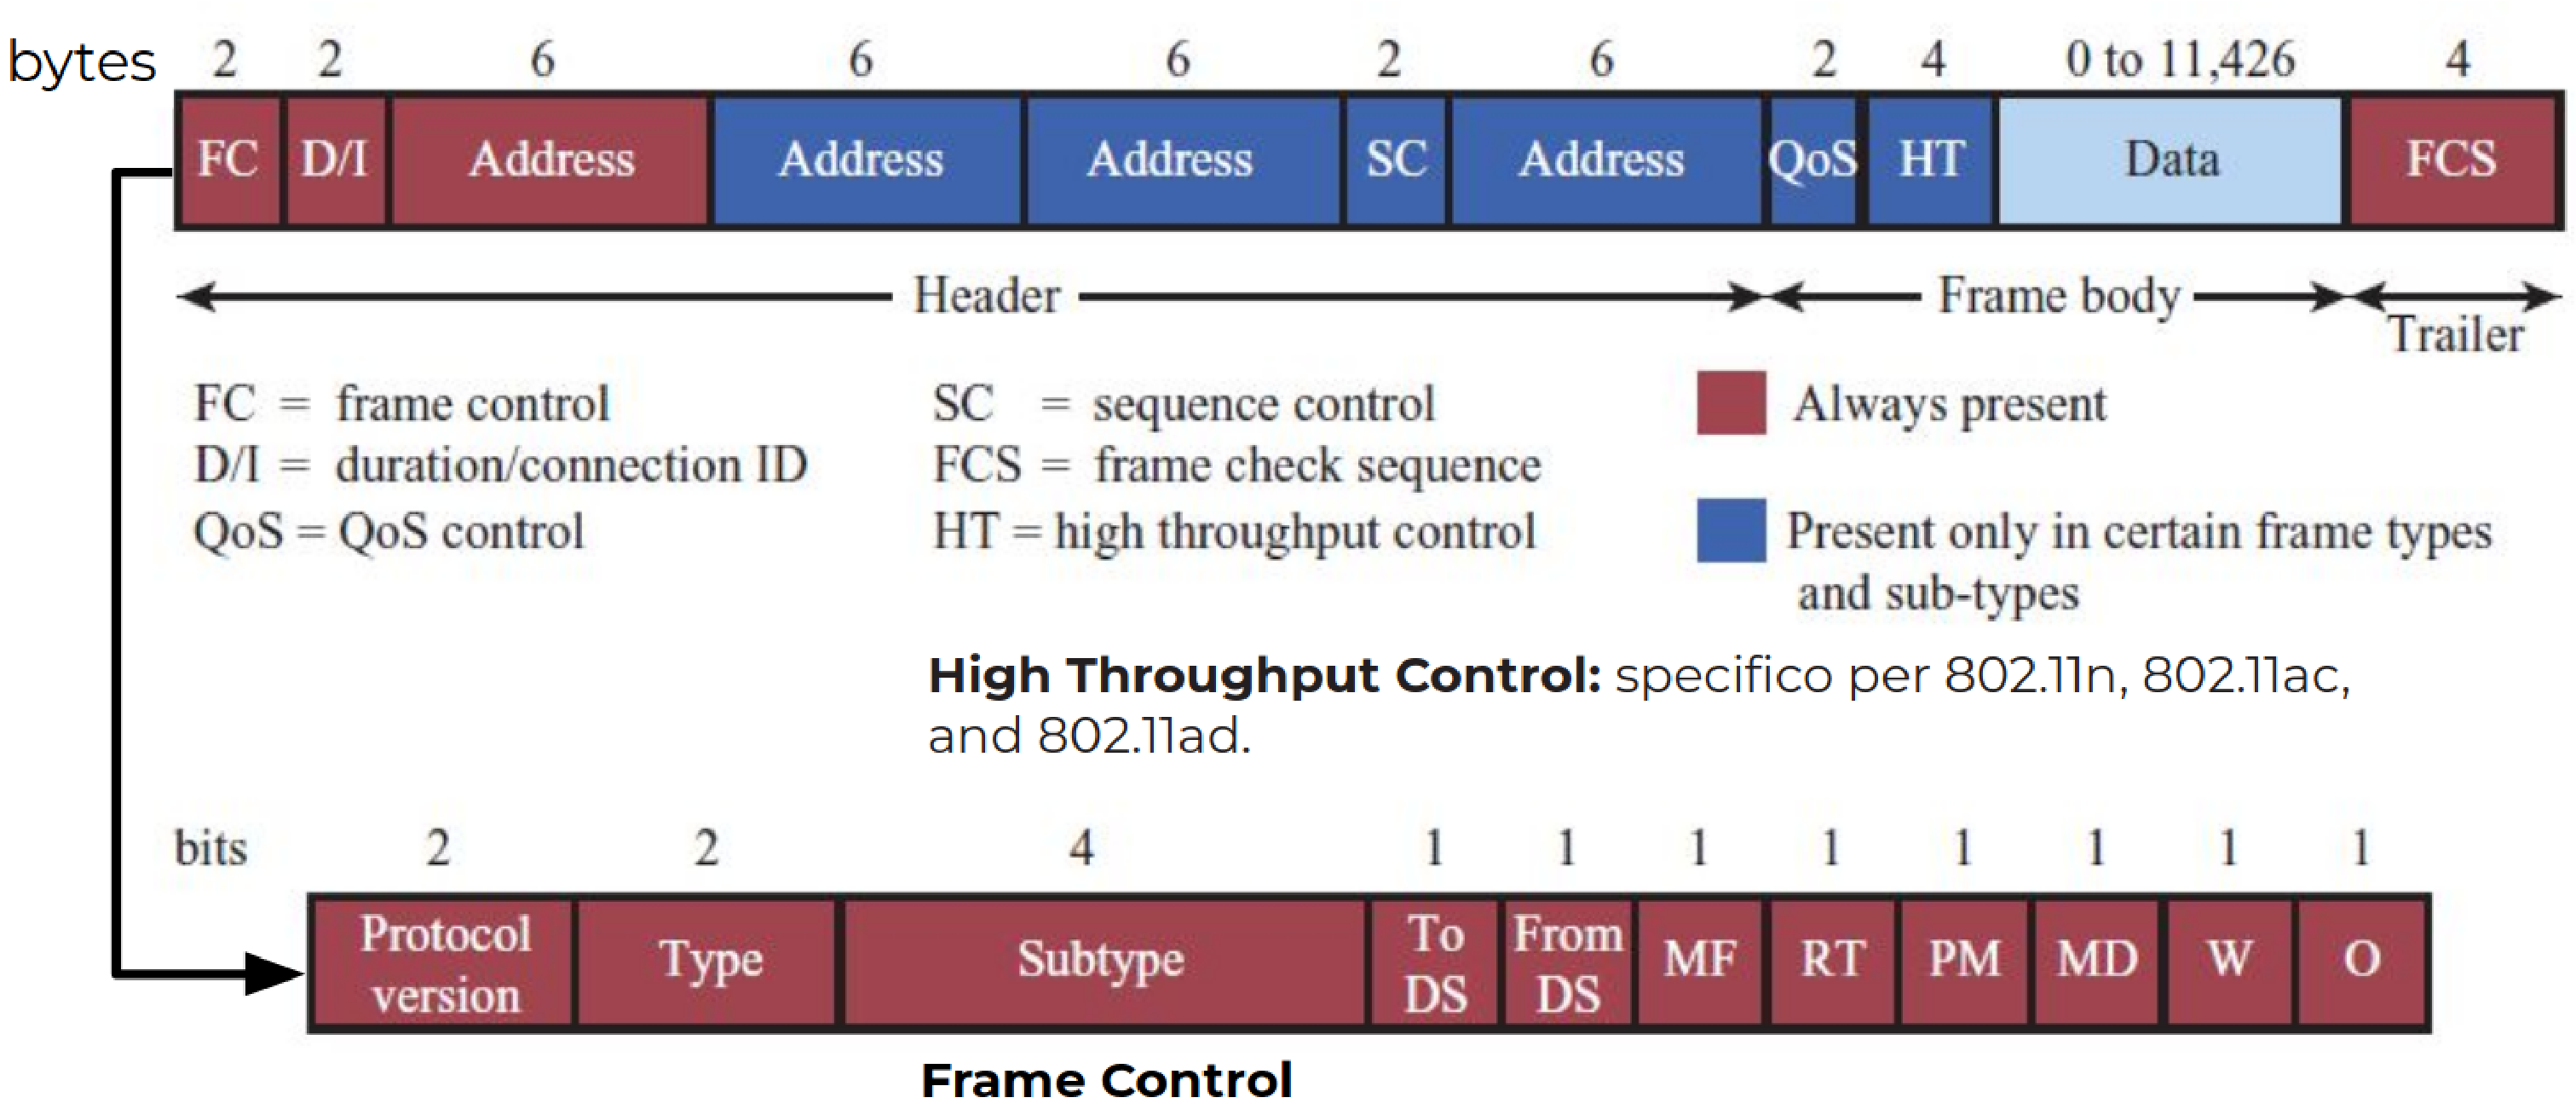
\includegraphics[width=0.9\linewidth]{img/wlan/macframe}
\end{center}

In rosso la parte sempre presente: in qualsiasi frame 802.11 sono presenti i campi in rosso. Gli altri sono presenti solo se necessari.

I primi 2 byte sono \textbf{Frame Control FC}, il quale contiene:
\begin{itemize}
	\item Protocol version: versione del protocollo

	\item 2 bit di Type

	\item 4 bit di sottotipo

	\item To DS/From DS sono bit che indicano se verso o dal Distributed System

	\item More Fragments MF: indica se c'è frammentazione

	\item Retry RT se si tratta di una retrasmissione

	\item Power Management PM per indicare se è attivo il risparmio energetico

	\item More Data MD se ci solo ulteriori dati

	\item 2 bit di controllo
\end{itemize}

Il secondo gruppo di 2 byte contiene la \textbf{Duration} o \textbf{Connection ID (D/I)}. Contengono la durata della trasmissione rimanente (in $\mu s$), usata per gestire i NAV. Nei frame Power Save Poll contiene l'Association ID del client che chiede informazioni.

Poi c'è l'\textbf{indirizzo di destinazione} del frame e \textbf{fino ad altri 3 indirizzi}, che possono esserci in base all'utilizzo; al termine del frame si ha una parte per la correzione degli errori. 

\paragraph{Frame Control:} Per quanto riguarda il tipo, ne esistono 3:
\begin{itemize}
	\item \texttt{00} Management

	\item \texttt{01} Controllo

	\item \texttt{10} Data
\end{itemize}

Sono macro-tipi che possono assumere i frame, per andare nello specifico bisogna guardare il sotto-tipo.  Ad esempio: nei frame di management \texttt{1000} sono i beacon, nei frame di controllo \texttt{1011} è una RTS mentre per i data frame \texttt{0101} indica un CF-Ack.

\paragraph{Indirizzi:} Possono esserci \textbf{fino a 4 indirizzi}, il cui significato cambia in base ai valori di To DS e From DS:

\begin{center}
	\renewcommand{\arraystretch}{1.5}
	\resizebox{\textwidth}{!}{  % Resize table to fit page width
		\begin{tabular}{|>{\centering\arraybackslash}m{1cm}|>{\centering\arraybackslash}m{1cm}|
				>{\centering\arraybackslash}m{2.5cm}|>{\centering\arraybackslash}m{2.5cm}|
				>{\centering\arraybackslash}m{2.5cm}|>{\centering\arraybackslash}m{2.5cm}|
				>{\centering\arraybackslash}m{2.5cm}|}
			\hline
			\textbf{To DS} & \textbf{From DS} & \textbf{Address 1} & \textbf{Address 2} & \textbf{Address 3} & \textbf{Address 4} & \textbf{Caso di utilizzo} \\
			\hline
			0 & 0 & \textbf{DA} \newline Indirizzo MAC destinazione & \textbf{SA} \newline Indirizzo MAC sorgente & \textbf{BSSID} \newline della cella/ random se ad hoc & - & Rete ad hoc \newline Rete con infrastruttura singola cella \\
			\hline
			0 & 1 & \textbf{DA} \newline Indirizzo MAC destinazione all'interno di BSSID & \textbf{BSSID} \newline della cella a cui la frame è destinata & \textbf{SA} \newline Indirizzo MAC sorgente & - & Frame inviata attraverso DS ad un AP all'interno della cella che possiede BSSID dell'address 2 \\
			\hline
			1 & 0  & \textbf{BSSID} \newline della cella destinazione & \textbf{SA} \newline Indirizzo MAC sorgente & \textbf{DA} \newline Indirizzo MAC stazione che sta ricevendo & - & Frame inviata attraverso DS ad un AP di una cella diversa BSSID dell'address 1 \\
			\hline
			1 & 1 & \textbf{RA} \newline Indirizzo AP destinazione all'interno di DS & \textbf{TA} \newline Indirizzo AP sorgente all'interno di DS &  \textbf{DA} \newline Indirizzo della stazione che sta ricevendo & \textbf{SA} \newline indirizzo della stazione che sta inviando &  Frame tra AP di celle differenti usando DS \\
			\hline
		\end{tabular}
	}
\end{center}

Le ultime 3 righe fanno riferimento alla casistica in cui sono presenti più celle e serve routing tra di queste. I casi sono:
\begin{itemize}
	\item \texttt{01} From DS, verso un AP all'interno della cella, letto nell'indirizzo 2

	\item \texttt{10} Verso il DS, indico cella e indirizzo di destinazione

	\item \texttt{11} Da e Verso il DS, devo sapere da dove arriva e dove inviare, oltre che indirizzo originale e finale (routing tra celle)
\end{itemize}

\subsection{Orthogonal Frequency Division Multiple Access OFDMA}

Si parla di WiFi 6, il quale utilizza \textbf{OFDMA}, sfrutta \textbf{subcarrier per fornire connettività a più dispositivi contemporaneamente}. Prima tutte le sottoportanti erano usate per un dispositivo alla volta (OFDM, dove M sta per Multiplexing). Con OFDMA c'è la possibilità di fornire gruppi di canali diversi a dispositivi diversi. 

Usando OFDM con TDMA potrebbe esserci una situazione tipo
\begin{center}
	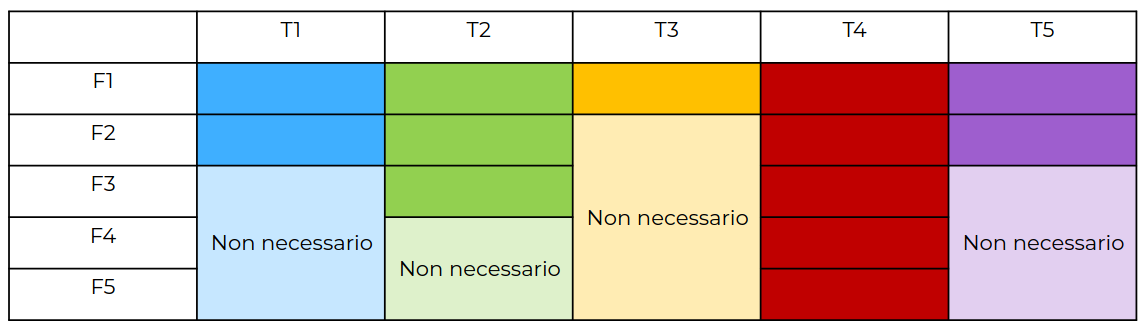
\includegraphics[width=0.75\linewidth]{img/wlan/tab1}
\end{center}
E dato che utenti diversi avranno necessità diverse questo potrebbe portare a "sprecare" frequenze. 

Con OFDMA si può avere arrivare a una situazione come
\begin{center}
	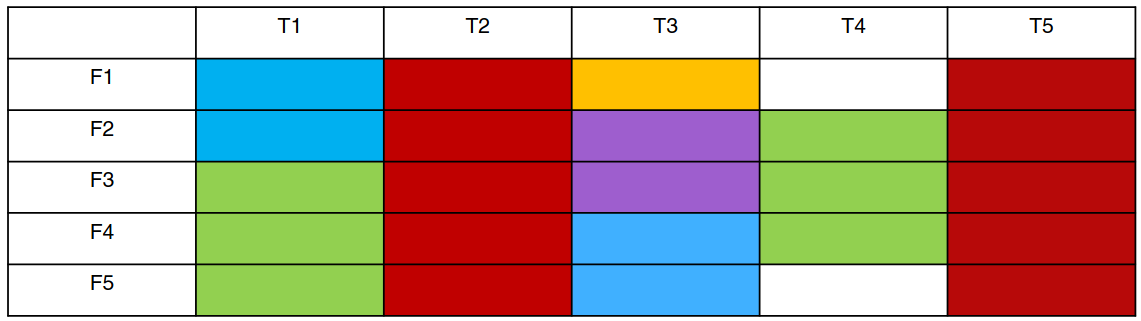
\includegraphics[width=0.75\linewidth]{img/wlan/tab2}
\end{center}

Vengono serviti \textbf{più dispositivi allo stesso momento}, gruppi di sottoportanti vengono assegnate a dispositivi diversi. Facendo questo si complica lo scheduling: al posto di assegnare solo lo slot di tempo bisogna assegnare tempo e gruppo di frequenze.

Serve definire quanto e in quale modo le frequenze possono essere raggruppate. Con \textbf{Resource Unit RU} si intende il gruppo di frequenze (solitamente adiacenti) allocabili ad un utente, l'unità base di suddivisione della banda. Si assegnano "blocchi" di risorse ad ogni utente. La dimensione delle RU è variabile e dipende dalla banda disponibile e come l'AP vuole allocare le risorse agli utenti.

Le possibili RU per una banda di 20MHz divisa in sottoportanti da 78.125kHz sono 256 e si possono dividere come:
\begin{center}
	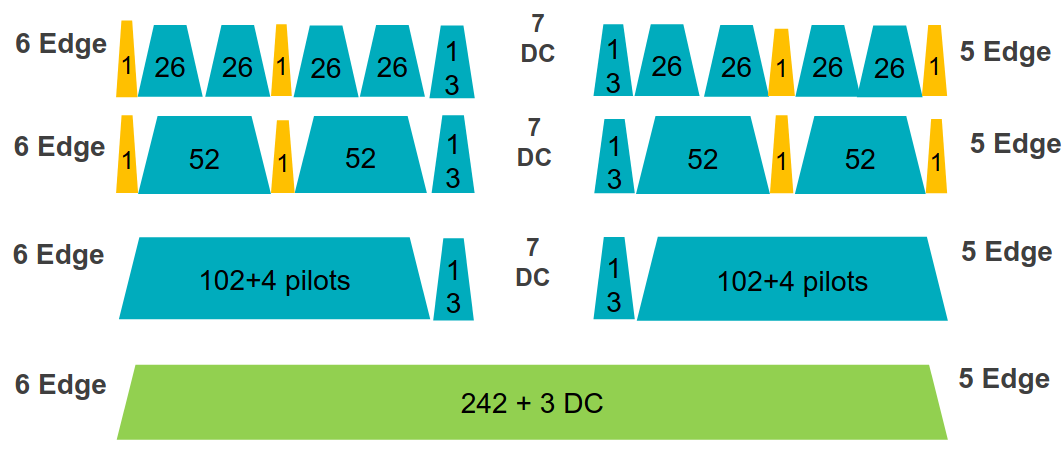
\includegraphics[width=0.8\linewidth]{img/wlan/ru1}
\end{center}

Non tutta la banda viene usata: sono presenti intervalli di guardia. Alcune sotto-portanti sono usate come \textbf{pilot}, trasmettono un'onda definita nello standard, in modo da permettere di stimare la qualità del canale e capire come effettuare la correzione del segnale. Vengono ripetuti "\textit{ogni tanto}" per rifare la misura.

L'AP deve usare frame di controllo: alcuni sono nuovi a 802.11ax per supportare le nuove funzionalità, altri già presenti nelle precedenti versioni.

Le informazioni di allocazione delle RU sono usate dai livelli PHY e MAC. Ogni risorsa è identificata da una sequenza unica di 7 bit, ad esempio:
\begin{center}
	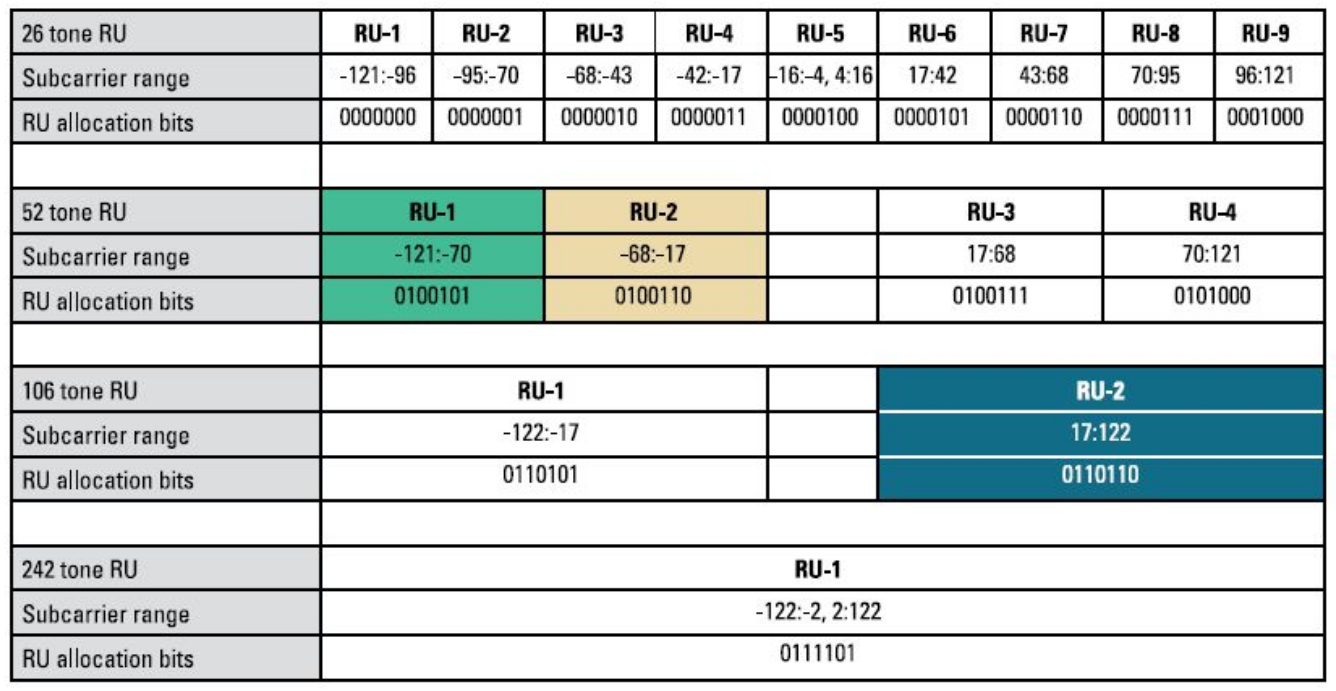
\includegraphics[width=0.975\linewidth]{img/wlan/tab3}
\end{center}

Ciascun codice rappresenta un \textbf{insieme di sottoportanti} e il numero indica il range di sottoportanti usate da quella RU. I codici sono tutti diversi, ognuno di questi identifica univocamente una RU e viene usato per indicare al dispositivo che frequenze utilizzare.

Una volta assegnata una risorsa, quelle al di sopra (per come rappresentate nella tabella) non possono essere utilizzate (hanno risorse in comune, gli insiemi di risorse devono essere mutualmente esclusivi); per il resto si può fare mix and match come è più comodo (non si è limitati ad usare lo stesso "livello" di RU).

\subsubsection{Downlink DL-OFDMA}

L'AP possiede dati da trasmettere e conosce la lista dei destinatari, ma deve anche comunicare l'assegnamento delle risorse. 
\begin{center}
	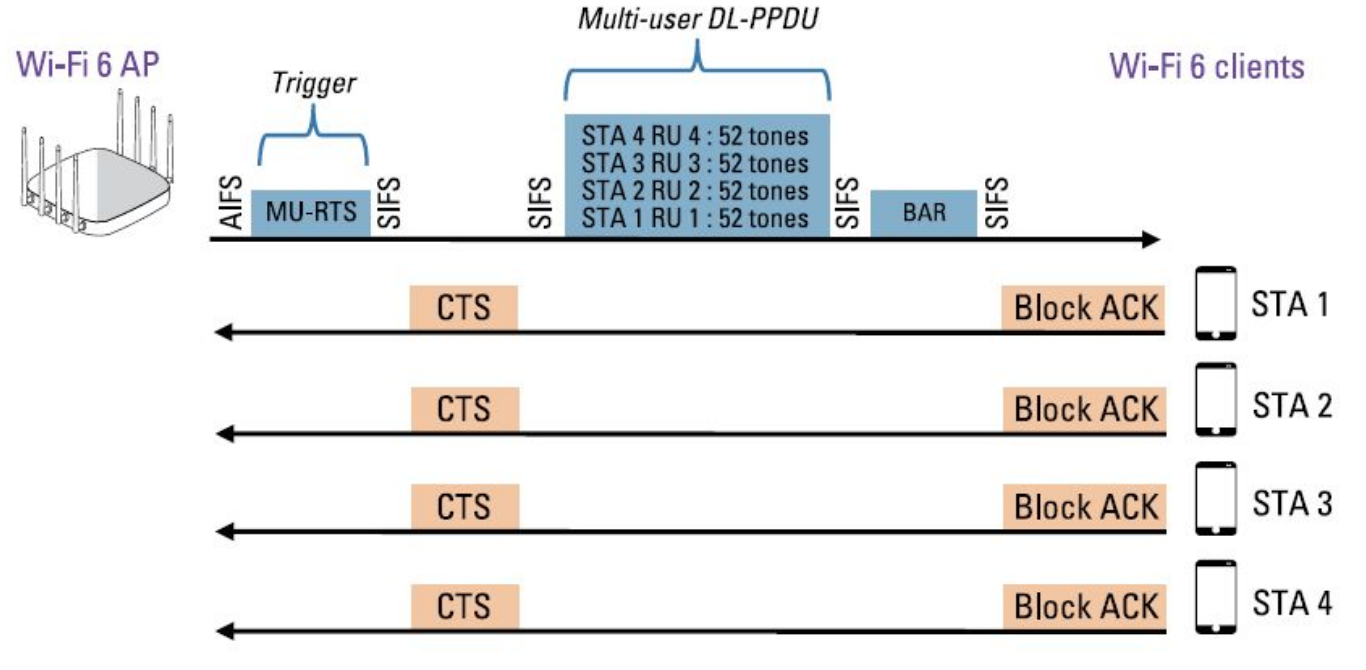
\includegraphics[width=0.95\linewidth]{img/wlan/downlink}
\end{center}

Viene usata una \textbf{Multi-User Request to Send MU-RTS}, un messaggio di controllo che ha il funzionamento di RTS e assegnamento delle risorse. Permette alle stazioni designate all'interno del messaggio di trasmettere, allo stesso tempo indicando alle altre di allocare il NAV.

In questo modo le stazioni possono essere a conoscenza delle risorse a loro dedicate e risponderanno con un CTS, in contemporanea (le frequenze sono ortogonali, non collidono). Per la risposta, ogni stazione ascolta solo la porzione di canale a lei associata.

Dopo il termine dei frame i dispositivi non mandano subito l'ack, ma l'AP aspetta SIFS e invia un \textbf{Block Acknowledgement Request BAR} ed i dispositivi rispondono in parallelo con un \textbf{Block ACK}.

Se gli ack fossero immediatamente al termine della trasmissione per ogni dispositivo l'ack potrebbe andare perso se l'AP non è ancora in modalità di ricezione.

L'ordine è
\begin{center}
    MU-RTS $\rightarrow$ CTS $\rightarrow$ Assegnamenti RU $\rightarrow$ BAR $\rightarrow$ ack
\end{center}
Ognuno di questi intervallato da tempo SIFS.

\subsubsection{Uplink UP-OFDMA}

L'uplink è \textit{meno prevedibile} e richiede di sincronizzare tutti i dispositivi che si vuole trasmettano contemporaneamente. 

La trasmissione deve avvenire in modo sincronizzato, dopo aver comunicato a ogni stazione la risorsa su cui trasmettere; il tutto coordinato dall'AP.
\begin{center}
	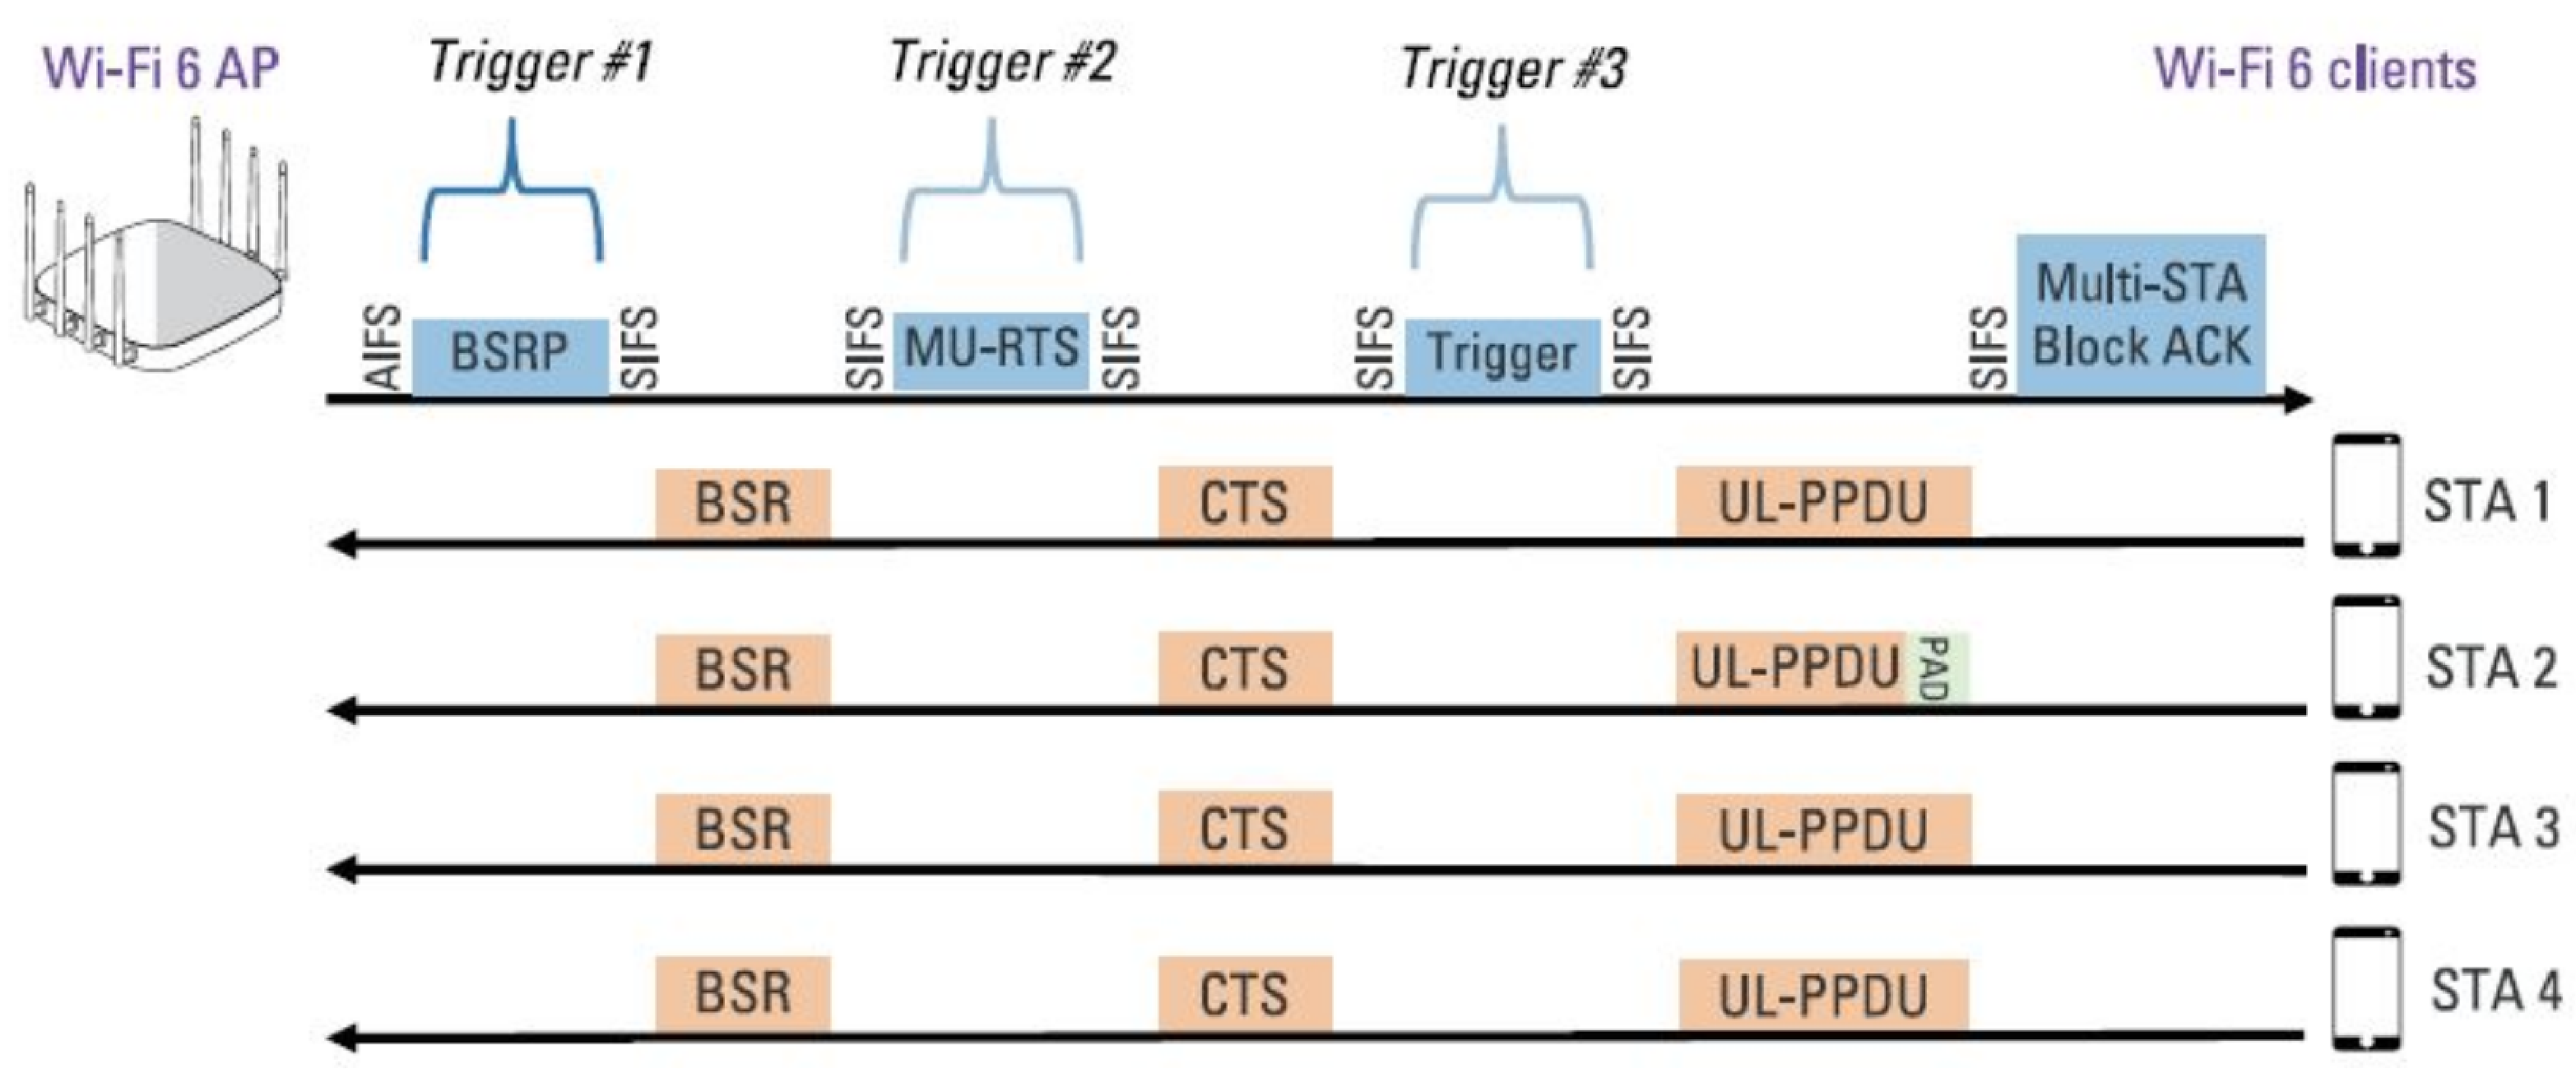
\includegraphics[width=0.95\linewidth]{img/wlan/uplink}
\end{center}

Ci sono più step:
\begin{itemize}
	\item \textbf{Buffer Status Report Poll BSRP}: l'AP chiede alle stazioni se hanno dati da trasmettere, in parallelo; interroga un sottogruppo di stazioni per chiedere chi ha da dire qualcosa
    
	\item I dispositivi rispondono con un \textbf{Buffer Status Report BSR}: le stazioni che hanno da trasmettere rispondono con una misura della quantità di dati (al fine di allocare le risorse)
	
    \item l'AP \textbf{assegna risorse} in base alle risposte delle stazioni e invia il \textbf{MU-RTS}, indicando la suddivisione delle RU
	
    \item Le stazioni rispondono con un \textbf{CTS}
	
    \item Poi è presente un \textbf{trigger aggiuntivo} da parte dell'AP, per far sincronizzare i dispositivi; tutte le stazioni devono trasmettere nello stesso momento (ad esempio tenendo in considerazione che chi è più lontano comincia prima)
	
    \item \textbf{Ogni stazione trasmette in parallelo} sulle risorse che gli sono state allocate; se la trasmissione di una stazione dura meno, questa fa padding
	
    \item Infine, se necessario, vengono inviati gli ack; \textbf{multi-station block acknowledgment Multi-STA Block ack} a tutte le stazioni che ne hanno fatto richiesta
\end{itemize}

% End L11

In banda $2.4GHz$ sono presenti \textbf{14 canali}, ma allo stesso tempo \textbf{non sovrapposti} possono essercene solo \textbf{3}.

\begin{center}
	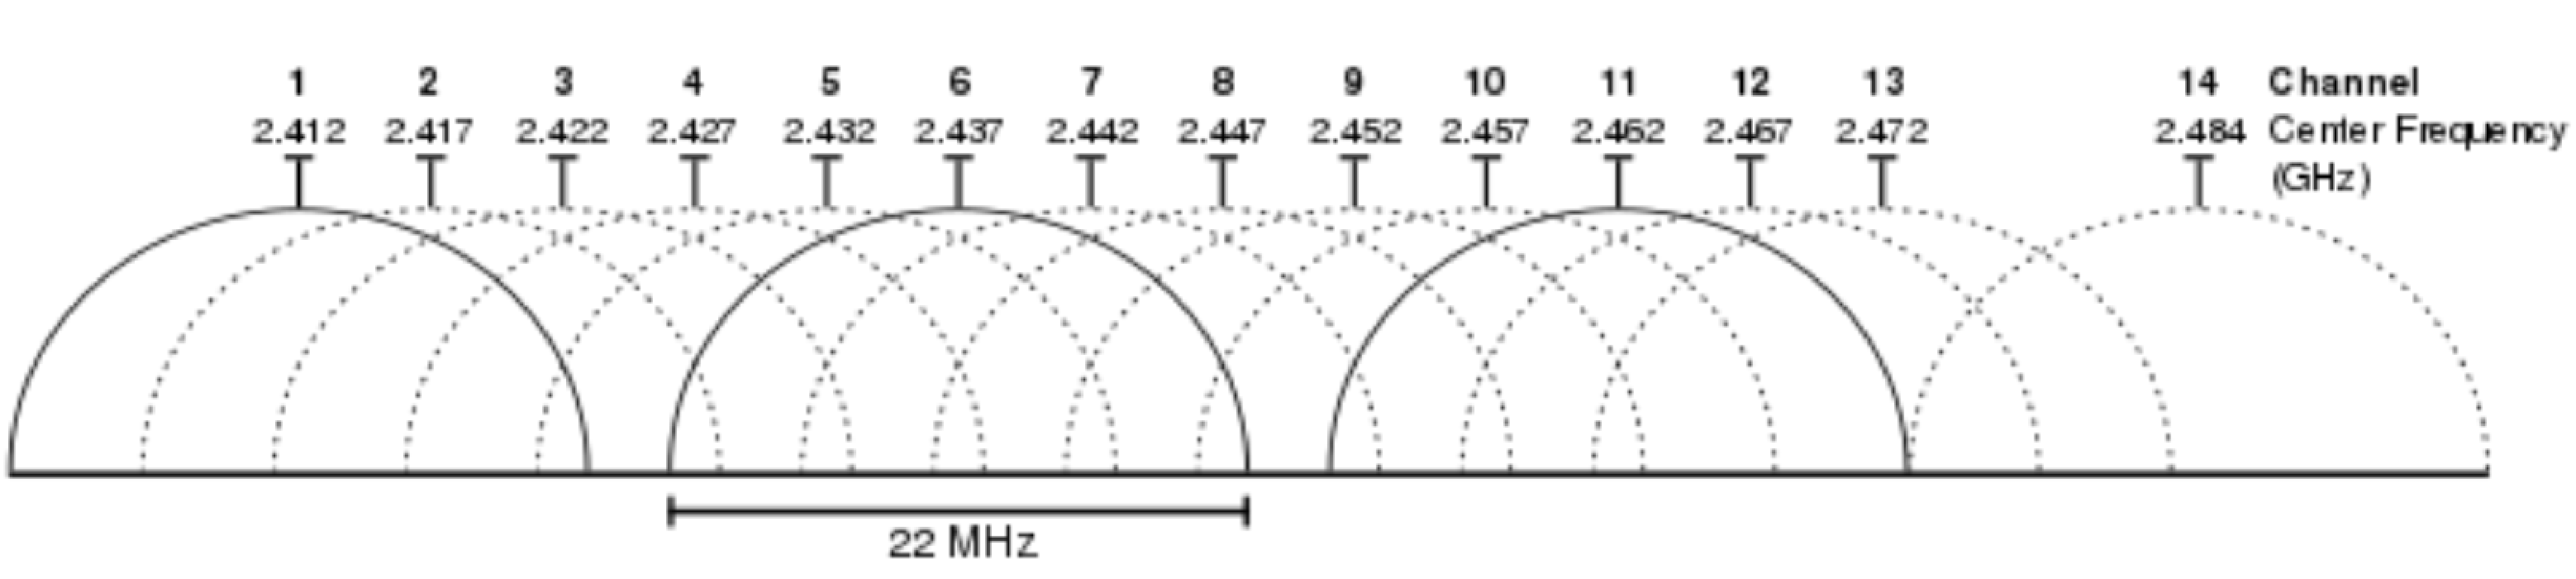
\includegraphics[width=0.99\linewidth]{img/wlan/24bande}
\end{center}
Insomma, se tutti usassero la stessa sarebbe un casino.

Per la banda $5GHz$ la configurazione è 
\begin{center}
	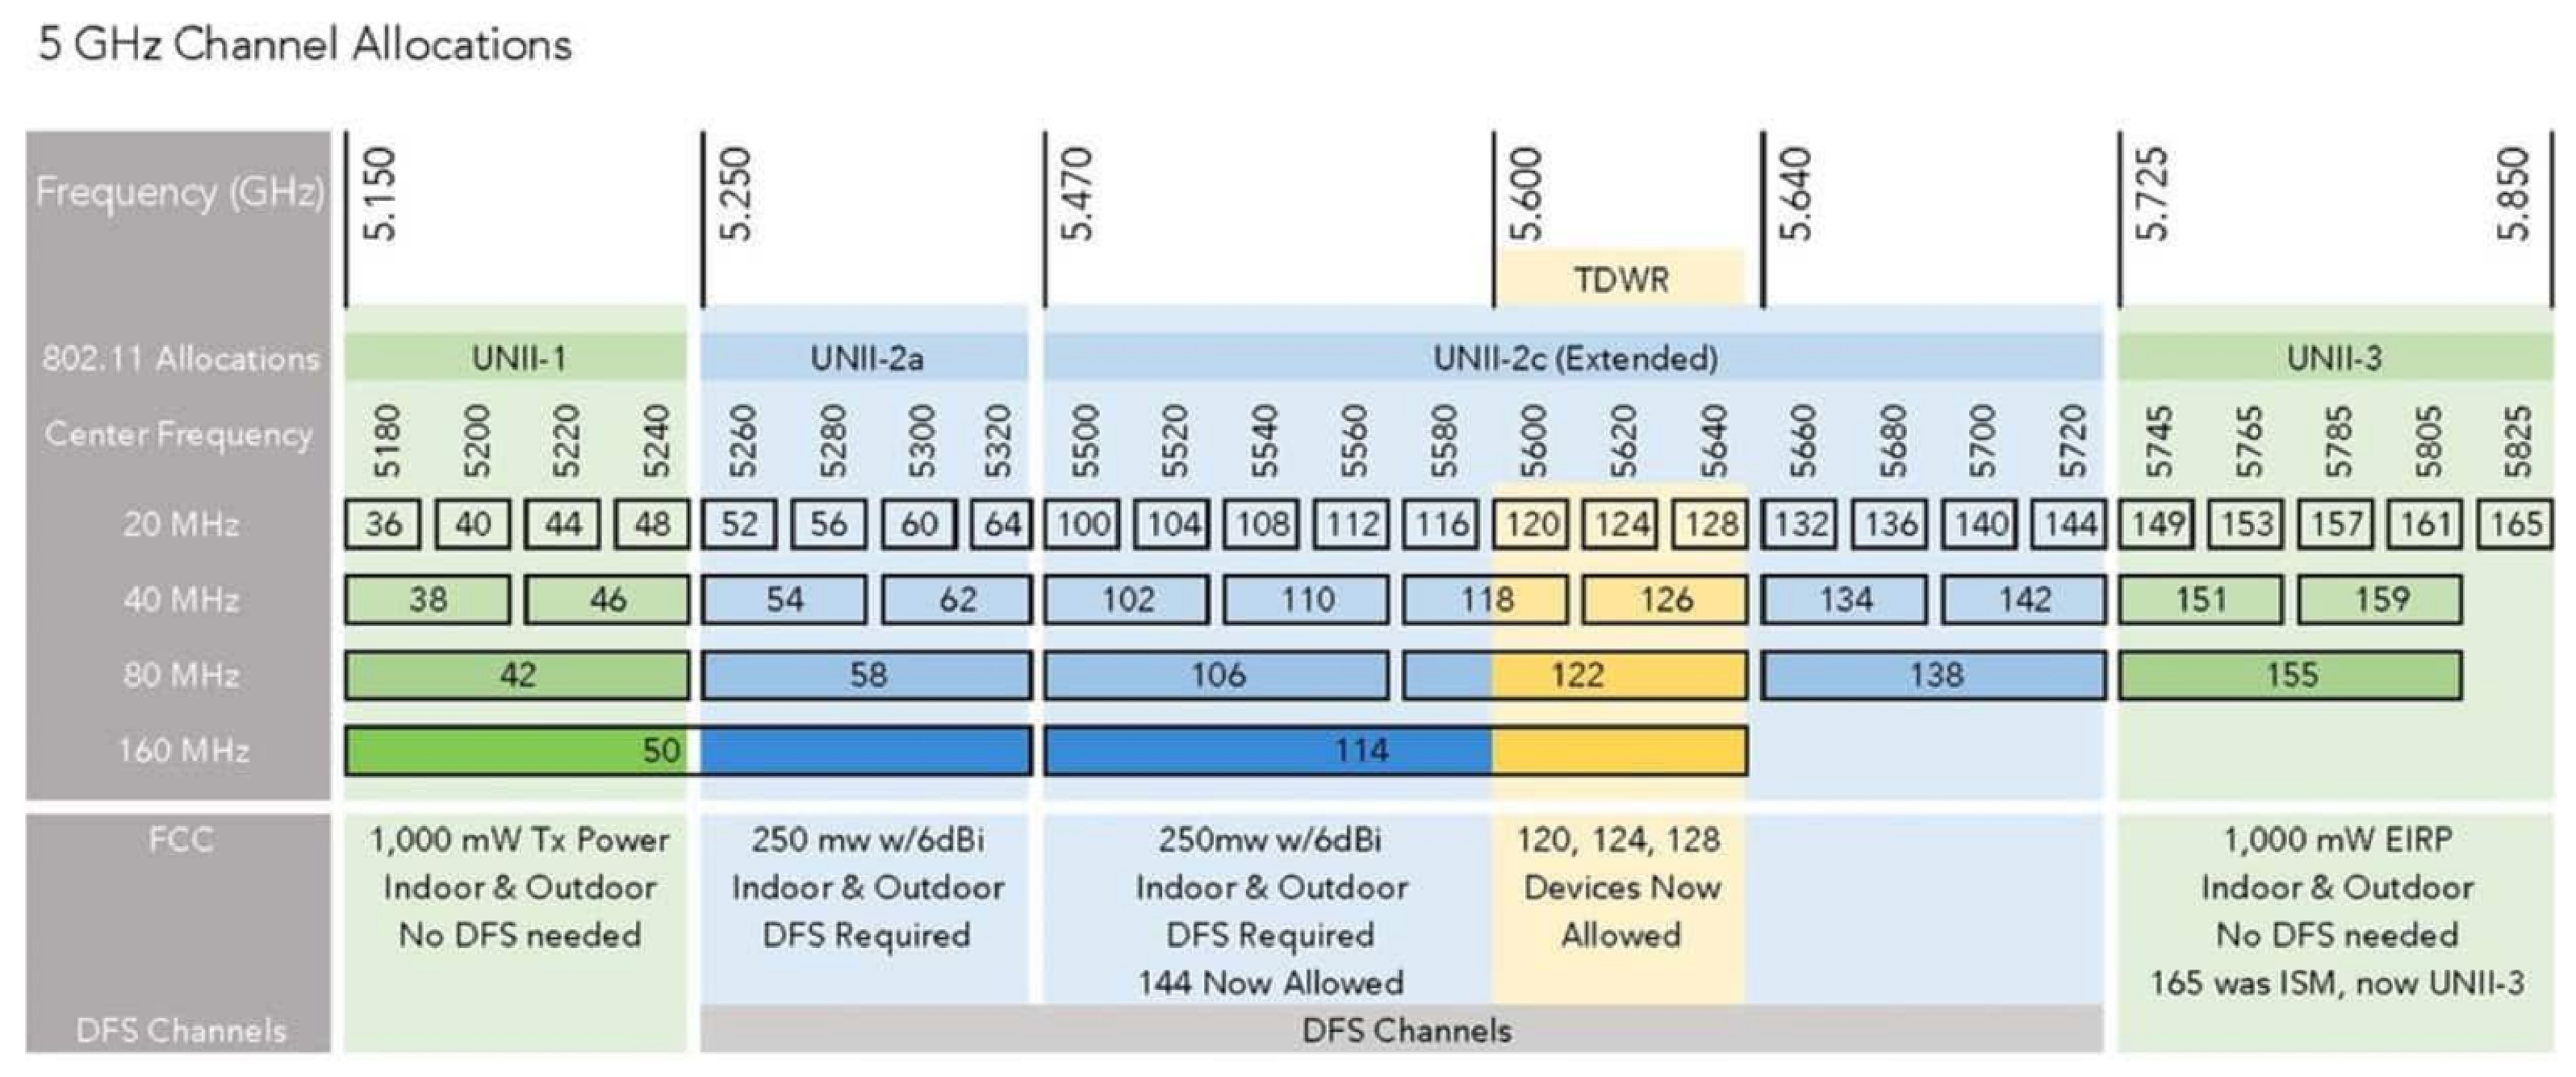
\includegraphics[width=\linewidth]{img/wlan/5bande}
\end{center}

Per ogni ampiezza di banda si ha una serie di range possibili, ognuno con il proprio identificatore. Nel momento in cui un dispositivo si deve connettere, all'interno del beacon si trova l'informazione sul canale utilizzato. All'interno di questi canali ci sono le sottoportanti.

\subsection{WLAN Security}

All'interno di 802.11 sono definite delle feature per la sicurezza. Per definizione il canale radio è \textit{molto} esposto, tutti possono ascoltare/inviare su un canale intrinsecamente broadcast. Di conseguenza si ha la necessità di cifrare il canale anche a livello di data link.

\paragraph{Wired Equivalent Privacy WEP:} Caratteristiche:
\begin{itemize}
	\item Algoritmo di cifratura RC4

	\item Opzionale, non è obbligatorio attivarlo

	\item Assenza di un sistema di gestione delle chiavi, tutto il traffico era cifrato allo stesso modo (la chiave non è la password wi-fi)

	\item Tutto il traffico viene cifrato con la stessa chiave
\end{itemize}

\paragraph{Robust Security Network RSN:} Per sopperire alle lacune di WEP è stato introdotto un emendamento allo standard, 802.11i. Viene definito il RSN, con al suo interno diversi servizi:
\begin{center}
	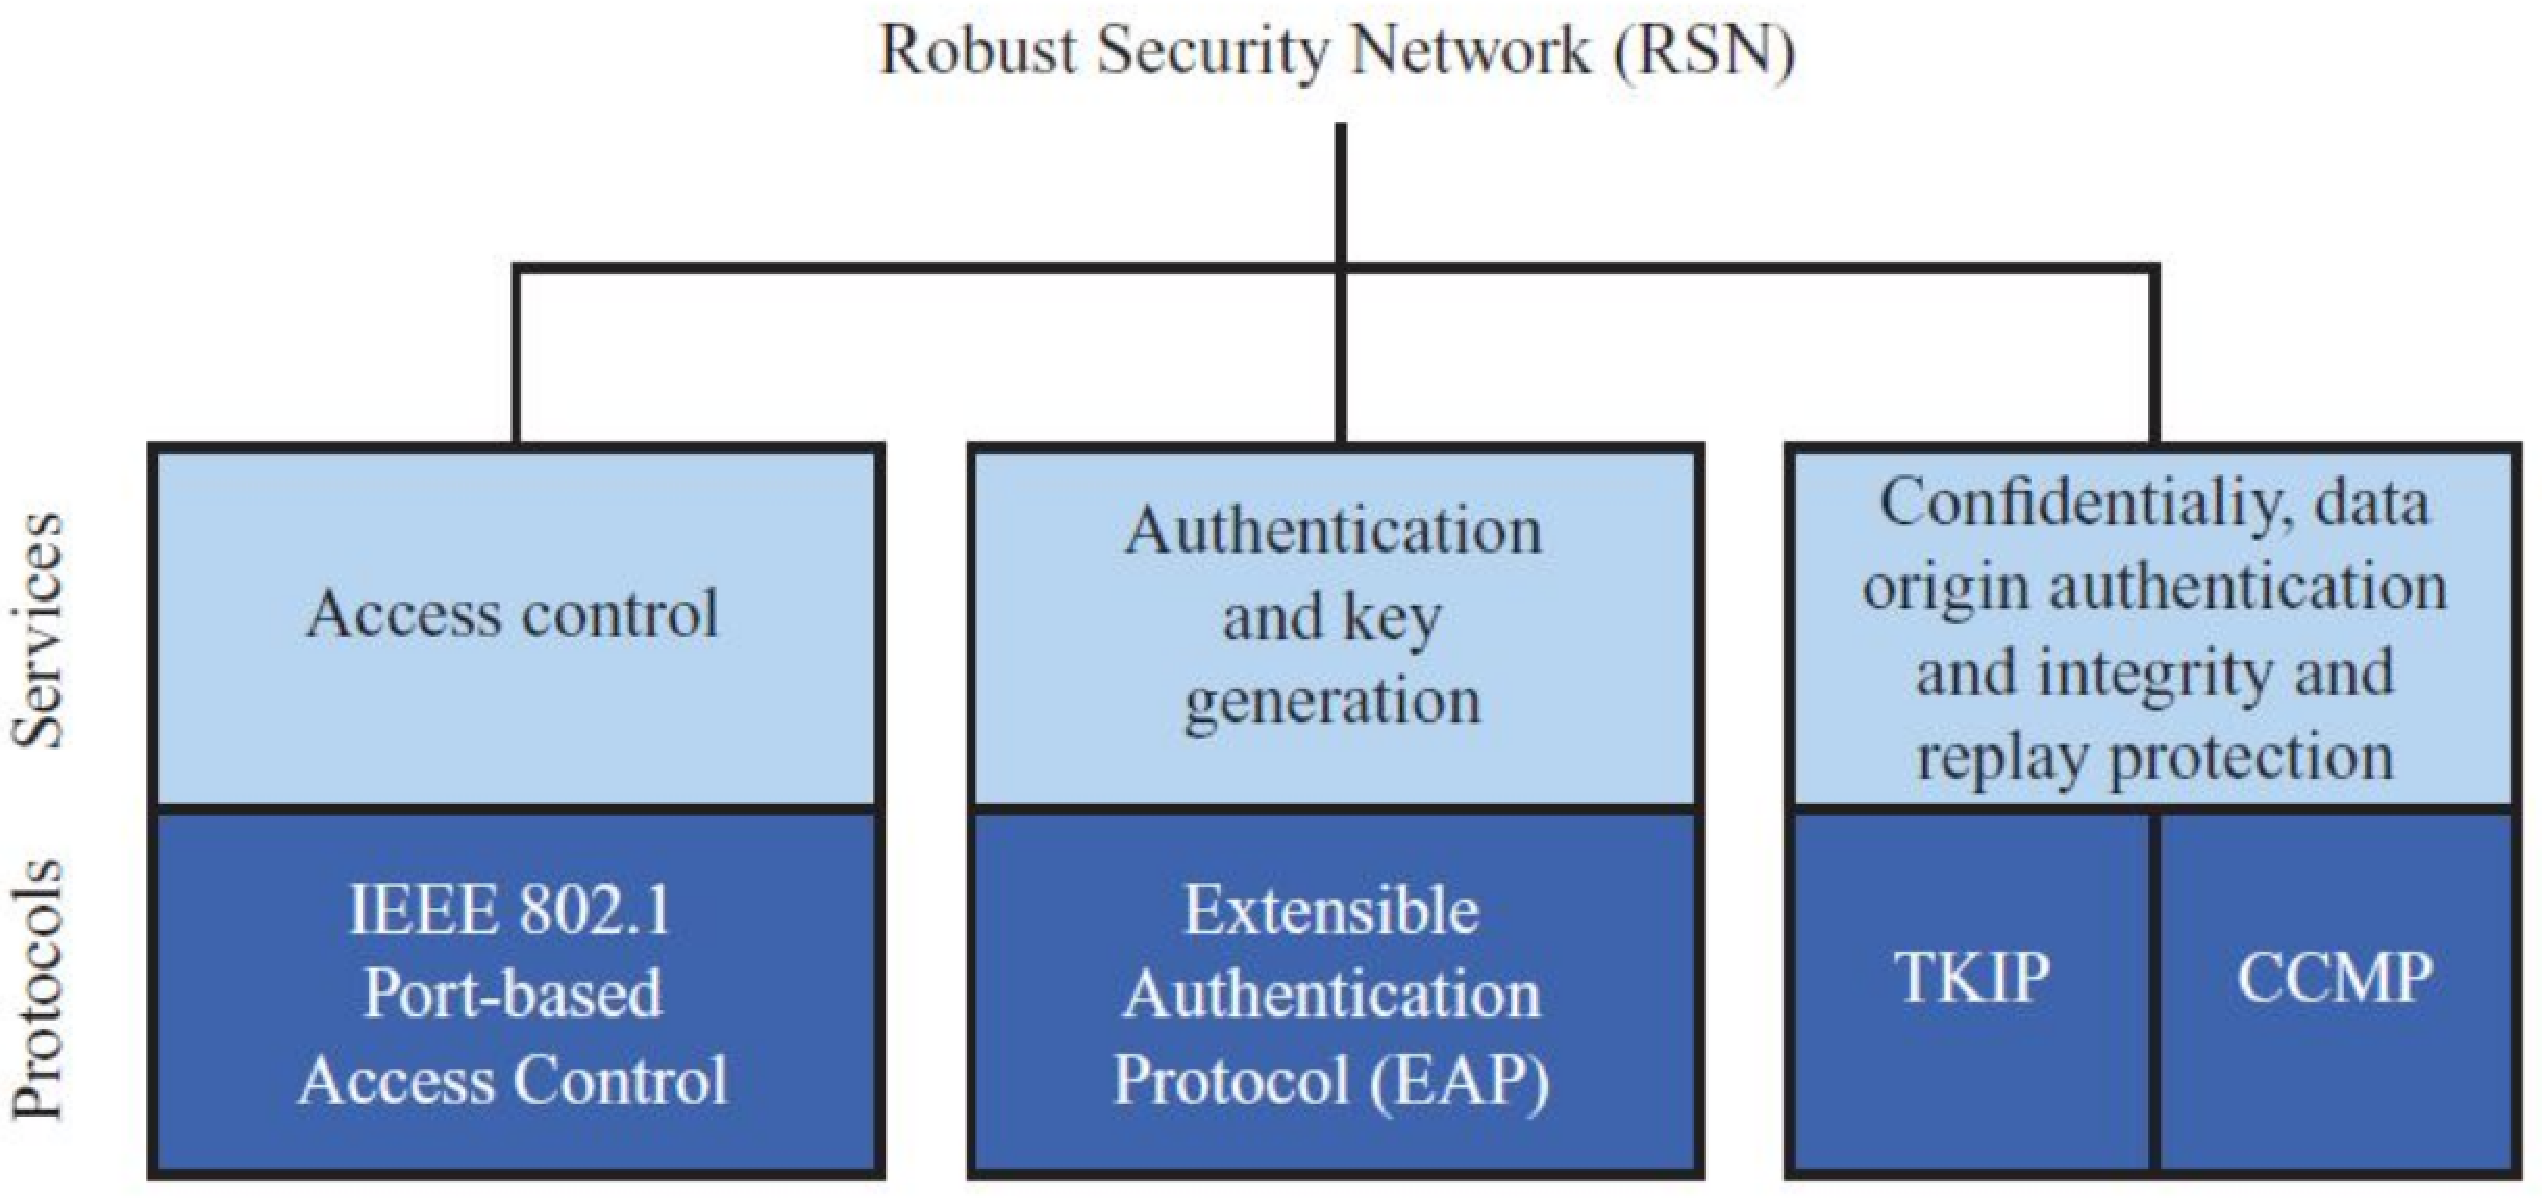
\includegraphics[width=0.7\linewidth]{img/wlan/rns}
\end{center}
\begin{itemize}
	\item \textbf{Access control}: impone l'utilizzo di protocolli di sicurezza e assiste lo scambio delle chiavi

	\item \textbf{Authentication}: definisce lo scambio tra utente e Authentication Server AS e genera le chiavi temporanee per la comunicazione sul canale radio

	\item \textbf{Privacy with message integrity}: il payload MAC (LLC PDU) viene cifrato (di più non posso altrimenti non so nemmeno per chi sia il messaggio, l'header MAC deve essere in chiaro) e viene aggiunto al messaggio una porzione dedicata al controllo dell'integrità
\end{itemize}

Ci sono più fasi per le operazioni:
\begin{itemize}
	\item \textbf{Discovery}: ovviamente il beacon non è cifrato
    
	\item \textbf{Authentication}: si evidenziano AP e Authentication Server, il quale può coincidere fisicamente con l'AP o meno.
	
    \item \textbf{Key management}: generazione delle chiavi specifiche per il singolo dispositivo
	
    \item \textbf{Protected data transfer}: una volta ottenuta la chiave, si comincia la comunicazione cifrata
	
    \item \textbf{Chiusura} della connessione
\end{itemize} 
\begin{center}
	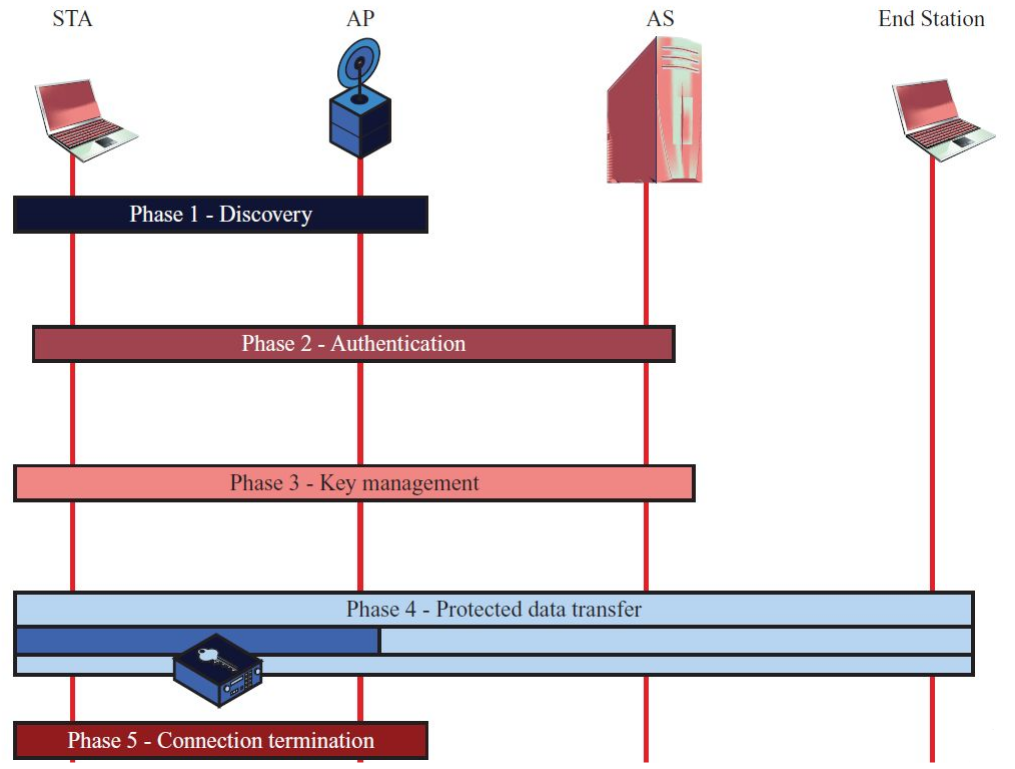
\includegraphics[width=0.95\linewidth]{img/wlan/fasop}
\end{center}

Nella fase di \textbf{discovery}: 
\begin{itemize}
	\item AP manda il beacon, il quale fornisce anche i servizi RSN disponibili (la modalità di accesso alla cella)
    
	\item La station STA dal beacon capisce quali sono i servizi RSN che può utilizzare (negoziano le capabilities di ognuno, si decide la policy da utilizzare)

	\item Associazione AP e STA, arrivano a un accordo sulle funzionalità di sicurezza da utilizzare. Può anche essere negata, da entrambe le parti (sia AP che STA possono decidere di negare la connessione)
\end{itemize}

Durante la fase di \textbf{autenticazione} e \textbf{gestione chiavi}: 
\begin{itemize}
	\item STA richiede ad AP autenticazione tramite la comunicazione con un Authentication Server AS
	
    \item Il server può essere remoto in caso di utilizzo di Extensible Authentication Protocol EAP
	
    \item Consegna delle chiavi in modo sicuro e generazione delle chiavi: viene generata una master key (a partire dalla password del WiFi) che viene usata per generare le altre chiavi crittografiche, richieste in seguito (lo standard non definisce come avviene lo scambio, si affida a EAP)
\end{itemize}

Come vengono \textbf{generate le chiavi}:
\begin{itemize}
	\item viene inviato un nonce da AP a Client

	\item la chiave di sessione $K_S$ viene calcolata dal Client a partire dai MAC address, i nonce e la master key (generata a partire dalla password della rete)

	\item il client invia il suo nonce, assieme a un $MIC_S$, ovvero Message Integrity Check, dipendente dalla sessione (quindi, in parte, dalla session key)

	\item l'AP può calcolare la stessa $K_S$ del Client

	\item L'AP invia la chiave di gruppo $K_g$, cifrandola tramite la chiave $K_S$

	\item Il Client verifica che l'AP ha la $K_S$ calcolata in modo corretto

	\item Il Client risponde con un ack, cifrato con la $K_S$

	\item L'AP verifica che la chiave del Client sia corretta
\end{itemize}
\begin{center}
	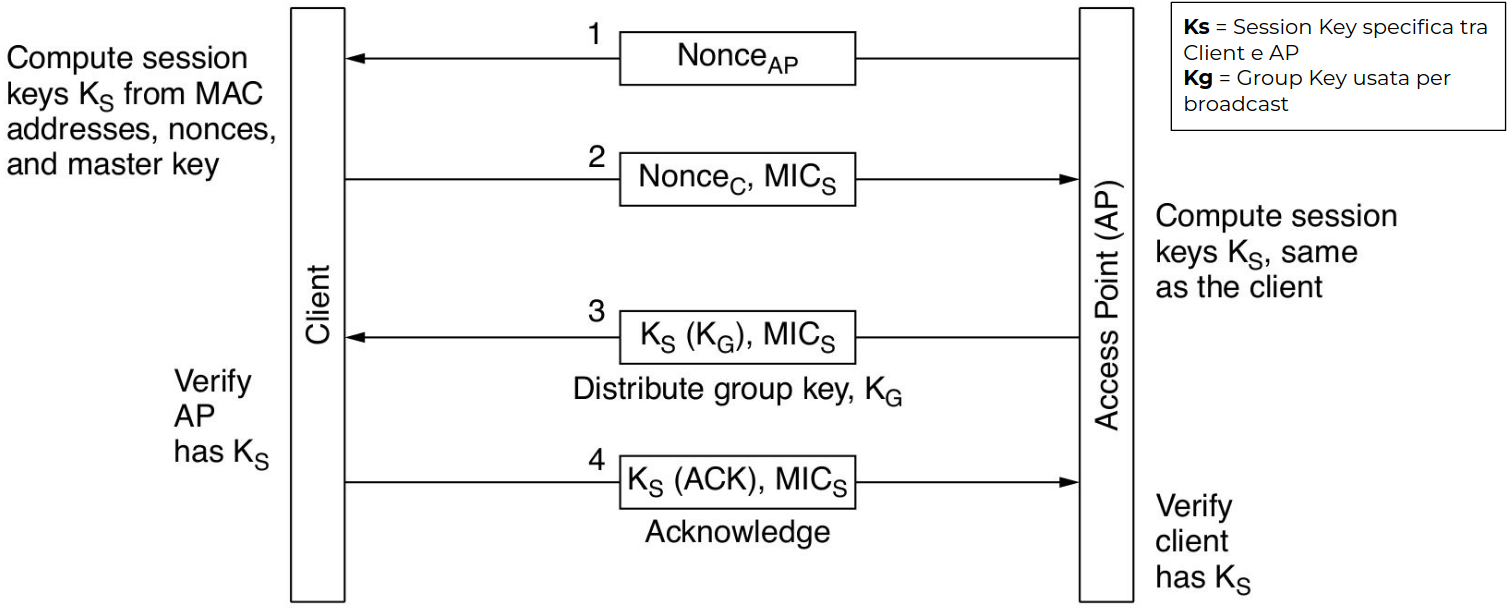
\includegraphics[width=0.98\linewidth]{img/wlan/keygen}
\end{center}

\paragraph{Protezione dati:} Lo standard 802.11i considera 2 alternative: 
\begin{itemize}
	\item \textbf{TKIP (WPA)}: aggiunge un codice di integrità 64 bit usando MAC di sorgente e destinazione; per la confidenzialità viene usato RC4; cambiamenti solo software rispetto a WEP

	\item \textbf{CCMP (WPA-2)}: integrità della cifratura tramite cipher-block-chaining CBC; integrità e confidenzialità tramite AES 128 bit
\end{itemize}

Tra i due cambia l'algoritmo di cifratura: per il primo non serviva cambiare nulla a livello hardware, per il secondo serve il supporto a CBC con AES.

Per la sicurezza: il segreto sta nella master key (il resto sarebbe pubblicamente accessibile), il presupposto è che l'attaccante non ne sia a conoscenza. Nelle varie versioni di EAP cambia il metodo con cui la chiave viene generata, per mantenere valido questo presupposto. Attacchi di tipo \href{https://it.wikipedia.org/wiki/Attacco_man_in_the_middle}{\texttt{MitM}} vengono evitati grazie ad integrity check e nonce.

\subsection{WiFi Protected Setup WPS}

Viene usato per evitare di mettere la password, su alcuni dispositivi in cui può essere comodo. All'interno del protocollo ci sono 3 tipi di dispositivi: 
\begin{enumerate}
	\item \textbf{Registrer}: entità che autorizza o revoca una stazione (AP o esterno)

	\item \textbf{AP}

	\item \textbf{Enrollee}: la stazione che vuole accedere
\end{enumerate}

Le \textbf{modalità di attivazione} sono in-band, due opzioni: 
\begin{itemize}
	\item \textbf{PIN}: può essere dell'AP da immettere sul dispositivo Enrollee, oppure dell'Enrollee da immettere sull'AP

	\item \textbf{Push Button}: pressione di un bottone su AP ed Enrollee, la procedura rimane attiva per massimo 2 minuti. Associazione FIFO (il primo che entra è autenticato)
\end{itemize}

\subsection{802.11e EDCA Enhanced Distributed Channel Access}

Altro emendamento allo standard, per aggiungere EDCA. Quando i livelli superiori richiedono un certo QoS viene migliorata la distribuzione dell'accesso al canale, modificando i parametri:
\begin{itemize}
	\item \textbf{CWMin}: Minima dimensione della contention window (numero random da aspettare)

	\item \textbf{CWMax}: massimo dimensione della contention window

	\item \textbf{AIFSN}: numero di SIFS$+$N slot time; definisce la lunghezza del tempo di attesa; il $+2$ è il minimo, equivalente a DIFS in totale (per definizione di DIFS)

	\item \textbf{Max TXPO}: massimo tempo nel quale una stazione può trasmettere più frame senza rilasciare il canale; quanto tempo la stazione può tenere il canale (0 vuol dire senza limite)
\end{itemize}

\begin{tabular}{|l|c|c|c|c|}
	\hline
	\textbf{Access Category} & \textbf{CWmin} & \textbf{CWmax} & \textbf{AIFSN} & \textbf{Max TXOP} \\ 
	\hline
	Background (AC\_BK) & 15 & 1023 & 7 & 0 \\ 
	\hline
	Best Effort (AC\_BE) & 15 & 1023 & 3 & 0 \\ 
	\hline
	Video (AC\_VI) & 7 & 15 & 2 & 3.008ms \\ 
	\hline
	Voice (AC\_VO) & 3 & 7 & 2 & 1.504ms \\ 
	\hline
	Legacy DCF & 15 & 1023 & 2 & 0 \\ 
	\hline
\end{tabular}

Si può vedere come per lo streaming video, e ancora di più per la voce, che la contention window viene ridotta, così come il tempo di attesa, ma il tempo massimo in cui possono occupare il canale è limitato. 

Le contention window delle varie categorie sono mutualmente esclusive, effettivamente creando un "ordine di priorità": voce, video, poi il resto.

Si tratta di una definizione più granulare delle politiche di accesso al canale in contesa, permettendo di ridurre i tempi per le applicazioni che ne necessitano.

%End L12

\subsection{802.11p \& Wave - V2V}

Si tratta di un WiFi "veicolare", rientra nelle \textbf{Dedicated Short-Range Communications DSRC} (con la banda dedicata $5.9GHz$). Serve per la comunicazione ad-hoc tra veicoli usando banda unlicensed.

Si tratta di una soluzione specifica, per il caso specifico: 
\begin{itemize}
	\item Rete \textit{altamente} dinamica

	\item Supporto alla guida autonoma (alert, dati sensori, ecc.; scambiati tra veicoli)

	\item Associazione veloce (dato che la rete è molto dinamica, non c'è troppo tempo)

	\item Supporto per servizi critici, come collisione (20ms), pedaggi (50ms), servizi a bordo strada (500ms), quindi con tempi anche molto ridotti

	\item Supporto infotainment
\end{itemize}

\subsubsection{Wireless Access for Vehiular Environment WAVE} 

Si tratta di un protocollo specifico per la situazione descritta prima, include una parte "normale" per il trasferimento di dati (TCP e famiglia), ma è presente anche una parte dedicata ai servizi necessari nell'ambito veicolare.
\begin{center}
	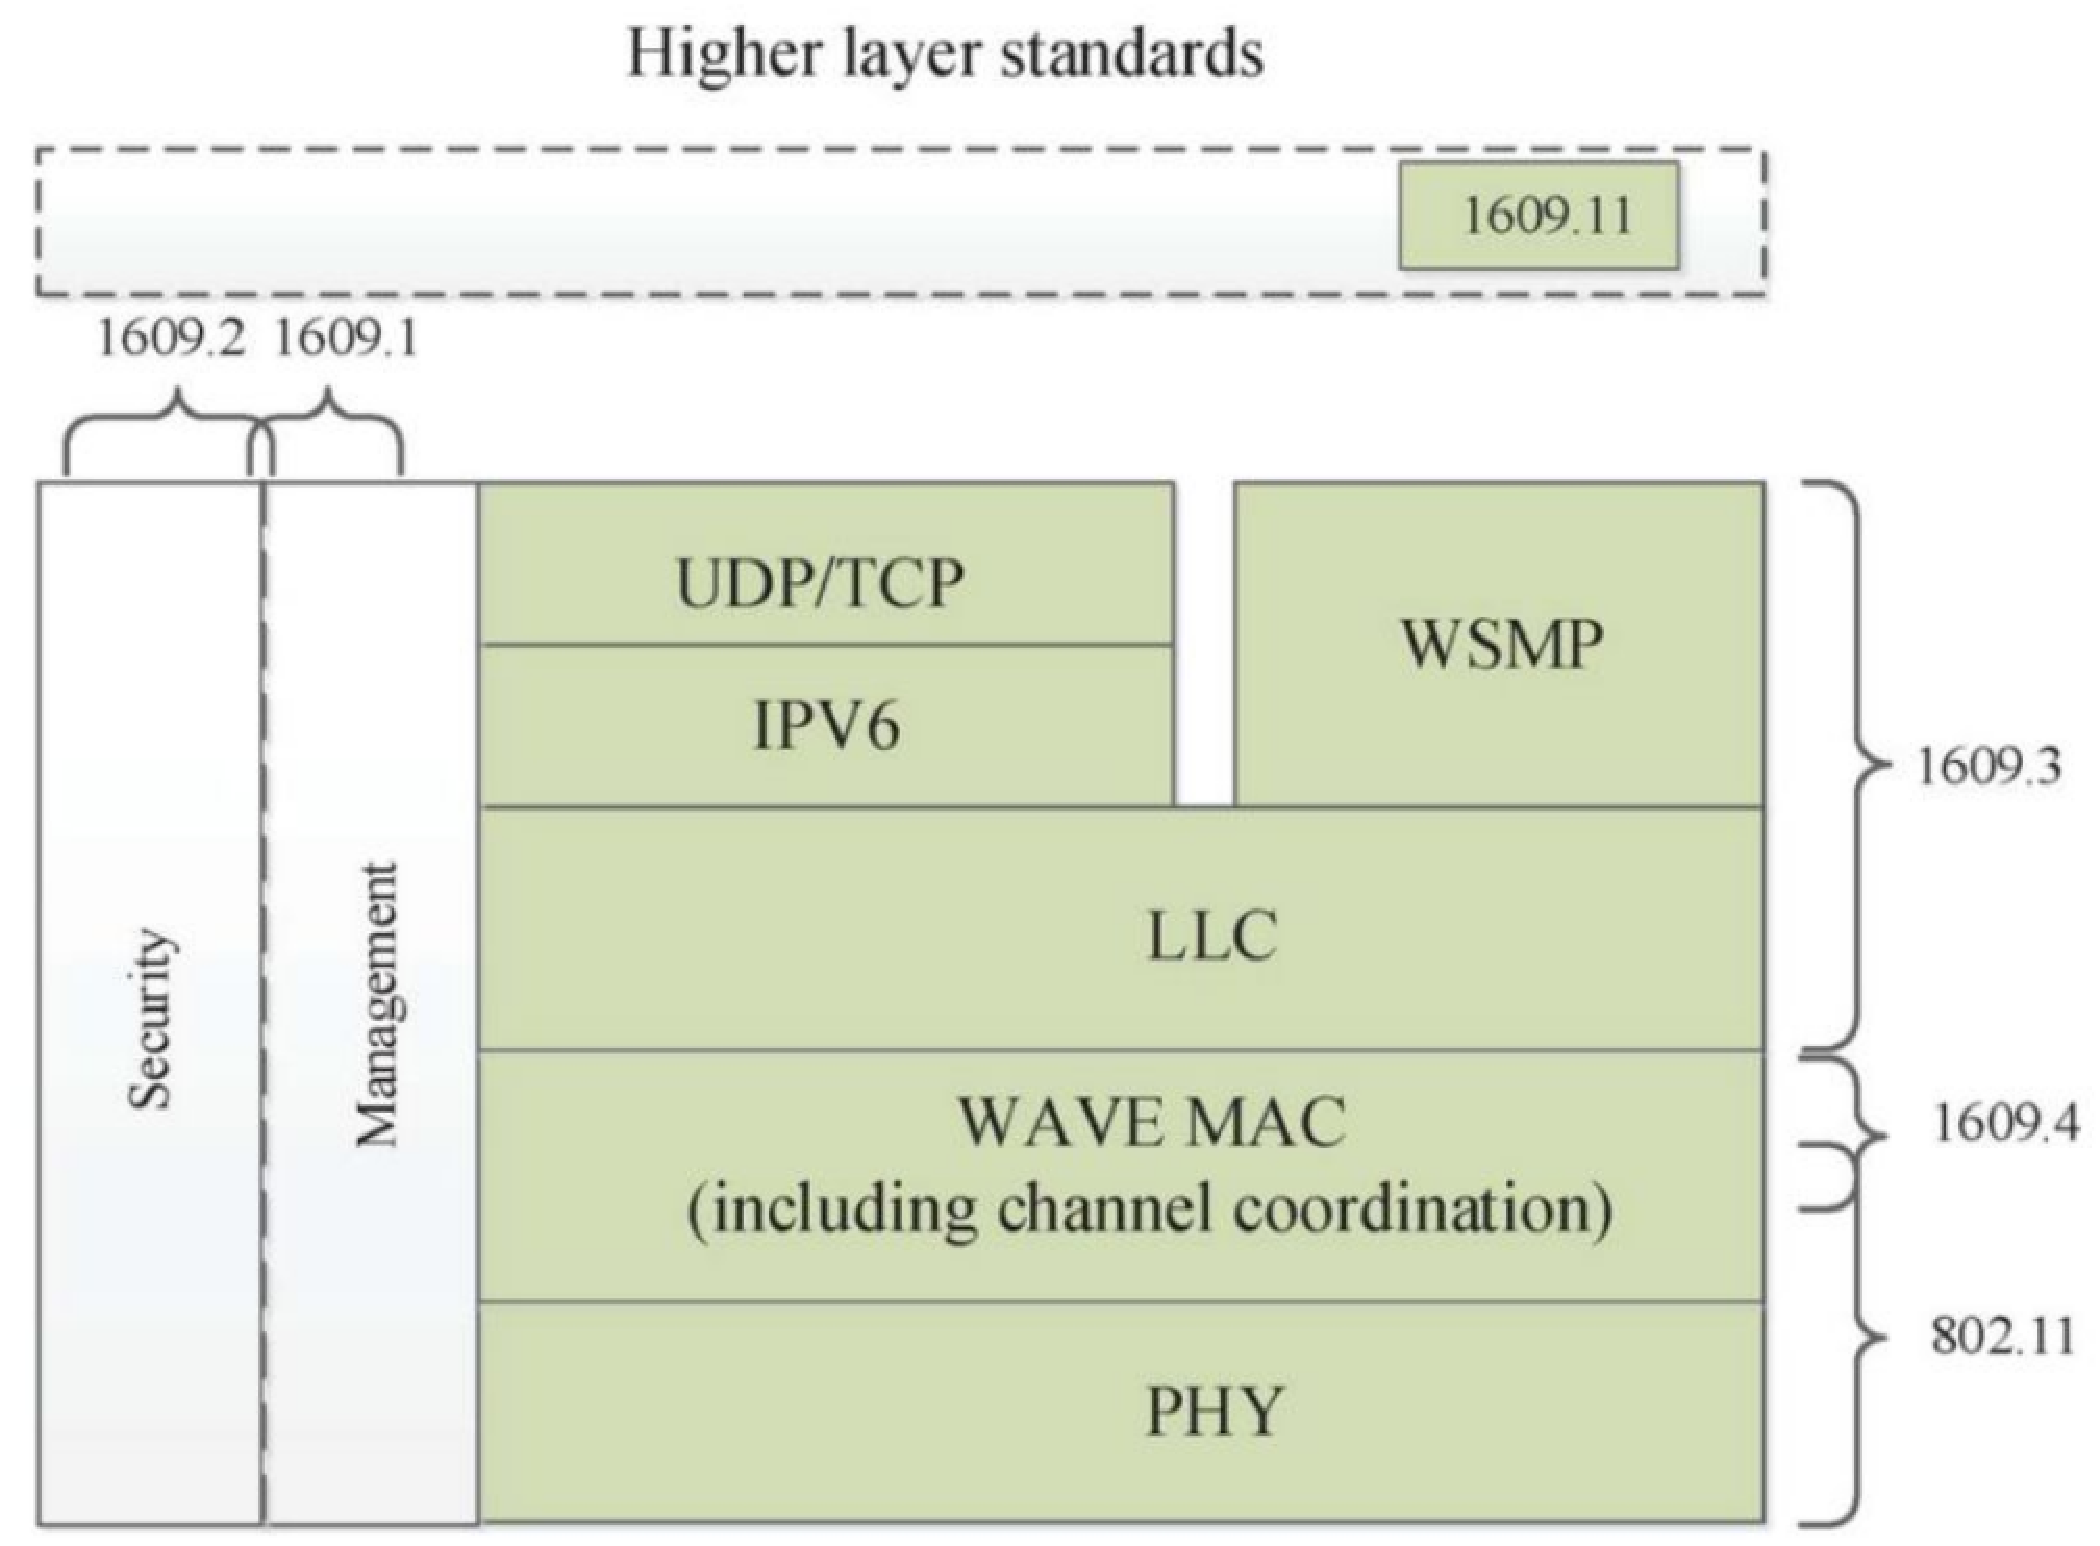
\includegraphics[width=0.75\linewidth]{img/wlan/wave}
\end{center}

Tutto lo stack si poggia sullo stesso standard IEEE (livello MAC e PHY), quindi viene usato l'emendamento 802.11e, che permette di gestire meglio diverse priorità a livello MAC.

Il canale fisico (802.11p) usa la banda $5.9GHz$ e permette diverse modulazioni e coding rate in base al range e quantità di informazioni richieste. Solitamente viene usato $QPSK$ $1/2$.

L'associazione deve essere molto veloce, quindi non sono previsti RTS e CTS.

%End slide WLAN1